\documentclass[11pt]{article}

\usepackage[margin=1in]{geometry}
\usepackage{amsmath,amssymb,amsthm,mathtools}
\usepackage{booktabs}
\usepackage{microtype}
\usepackage{tikz}
\usetikzlibrary{arrows.meta,positioning,calc,decorations.pathreplacing,fit,shapes.geometric}
\usepackage[hidelinks]{hyperref}
\usepackage[nameinlink,noabbrev]{cleveref}
\usepackage{enumitem}
\usepackage{array}
\usepackage{longtable}
\usepackage{xcolor}
\usepackage{graphicx}

\definecolor{tokblue}{HTML}{2E6FBB}
\definecolor{tokgreen}{HTML}{2D9A63}
\definecolor{tokamber}{HTML}{C9831A}
\definecolor{tokrose}{HTML}{B84A62}
\definecolor{tokgray}{HTML}{59616E}
\definecolor{toklight}{HTML}{F3F6FA}

\newtheorem{theorem}{Theorem}[section]
\newtheorem{lemma}[theorem]{Lemma}
\newtheorem{proposition}[theorem]{Proposition}
\newtheorem{corollary}[theorem]{Corollary}
\newtheorem{definition}[theorem]{Definition}
\newtheorem{assumption}[theorem]{Assumption}
\newtheorem{example}[theorem]{Example}
\newtheorem{remark}[theorem]{Remark}

\DeclareMathOperator{\softmax}{softmax}
\DeclareMathOperator{\argmax}{arg\,max}
\DeclareMathOperator{\conv}{conv}
\DeclareMathOperator{\Newt}{Newt}
\DeclareMathOperator{\Trop}{Trop}
\DeclareMathOperator{\Vtx}{Vert}
\DeclareMathOperator{\Aut}{Aut}
\DeclareMathOperator{\Hom}{Hom}
\DeclareMathOperator{\supp}{supp}
\DeclareMathOperator{\poly}{poly}
\DeclareMathOperator{\dist}{dist}
\DeclareMathOperator{\diag}{diag}
\DeclareMathOperator{\rank}{rank}
\newcommand{\R}{\mathbb{R}}
\newcommand{\N}{\mathbb{N}}
\newcommand{\Z}{\mathbb{Z}}
\newcommand{\Q}{\mathbb{Q}}
\newcommand{\one}{\mathbf{1}}
\newcommand{\Sn}{\mathfrak{S}_n}
\newcommand{\cG}{\mathcal{G}}
\newcommand{\cT}{\mathcal{T}}
\newcommand{\cX}{\mathcal{X}}
\newcommand{\cZ}{\mathcal{Z}}
\newcommand{\cY}{\mathcal{Y}}
\newcommand{\cD}{\mathcal{D}}
\newcommand{\cF}{\mathcal{F}}
\newcommand{\cP}{\mathcal{P}}
\newcommand{\cC}{\mathcal{C}}
\newcommand{\cR}{\mathcal{R}}
\newcommand{\cA}{\mathcal{A}}
\newcommand{\eps}{\varepsilon}
\newcommand{\tropadd}{\oplus}
\newcommand{\tropmul}{\odot}
\newcommand{\maxplus}{\mathbb{T}}
\newcommand{\bell}{\mathrm{Bell}}

\allowdisplaybreaks
\setlist[itemize]{leftmargin=1.5em}
\setlist[enumerate]{leftmargin=1.7em}

\title{\vspace{-1em}\textbf{Expressivity of Tokenized Graph Transformers: Tropical Geometry, Boolean Circuits, and Toric Fans}\\
\large Part II: How Edge--Vertex Tokenization Changes Transformer Expressivity}
\author{Amelie Schreiber}
\date{\today}

\begin{document}
\maketitle

\begin{abstract}
This paper develops a mathematical extension of the tropical-geometric theory of transformer expressivity to Tokenized Graph Transformers (TokenGT).  The starting point is the observation that the tropical limit of soft attention partitions query space by power diagrams and that multi-head attention refines the associated normal fans through Minkowski sums of Newton polytopes.  TokenGT changes this picture before any learned layer is applied: a graph is not represented as a bag of vertices, but as a sequence of vertex and edge tokens equipped with node identifiers and type identifiers.  This apparently simple change alters the relevant token count, the incidence information available to each attention head, the Boolean circuit primitives realizable by attention, and the polyhedral complex seen by the tropical skeleton.

We give a self-contained theory in five parts.  First, for fixed-size graphs and hypergraphs, we prove that TokenGT-style tokenization with order-$k$ identifiers yields universal approximation of continuous permutation-equivariant graph-to-graph maps, and exact interpolation of arbitrary finite graph-to-graph maps once labels or output slots are fixed.  The proof combines the equivariant-basis construction of TokenGT with invariant/equivariant graph-network universality and with a finite contextual-coding argument.  Second, we adapt circuit-complexity results for transformers: graph-token attention simulates threshold circuits over vertex and edge predicates, thereby separating TokenGT from ``naked'' graph transformers characterized by modal logics without structural encodings.  Third, we extend the tropical expressivity bounds: replacing node-only token count $n$ by graph-token count $N_G=n+m$ (or $n^k$ in dense order-$k$ form) changes the linear-region exponent from $\Theta(n^{dL})$ to $\Theta(N_G^{dL})$ under the same genericity assumptions, and exposes when edge tokenization yields no asymptotic gain.  Fourth, we analyze GraphCG-style latent steering.  We prove that the GraphCG objective does not by itself enlarge the formal architecture class, but biases TokenGT graph-to-graph maps toward controllable low-dimensional semantic flows; in the tropical skeleton, these flows are one-dimensional slices through the decoder fan.  Fifth, we analyze the toric geometry of ReLU networks.  We show that transformers meet toric geometry only through restricted polyhedral skeletons: unbiased rational ReLU subnets and conditioned zero-temperature attention give rational fans and Cartier support functions, but finite-temperature softmax, full self-attention with moving keys, biases, normalization, and signed values obstruct a general toric-variety theorem.  We give explicit counterexamples.  The result is a rigorous, didactic account of how TokenGT changes transformer expressivity from functional, circuit, training, tropical, and toric perspectives.
\end{abstract}

\tableofcontents
\newpage

\section{Introduction}

Transformer expressivity has several mathematically distinct meanings.  Universal approximation theorems ask whether a model class can approximate continuous sequence-to-sequence maps on compact sets.  Formal-language and circuit-complexity theorems ask what Boolean functions or languages can be recognized as input length grows.  Graph-learning theorems ask what graph invariances are respected and which graph properties survive relabeling.  Tropical geometry asks how attention and ReLU pieces partition a continuous domain into polyhedral cells, and how many such cells can be realized.  Toric geometry, in a newer ReLU-network formulation, asks whether the piecewise-linear function computed by a network is the support function of a divisor on a fan.

The present paper studies the interaction of these viewpoints for graph transformers, and in particular for TokenGT \cite{kim2022tokengt}.  TokenGT represents a graph by treating vertices and edges as independent tokens.  Each token is augmented with two types of structural information: orthonormal node identifiers that encode incidence through dot products, and trainable type identifiers that distinguish vertices from edges.  A standard transformer encoder then operates on this sequence.  The striking point, both theoretically and practically, is that the architecture remains a pure transformer; the graph inductive bias is moved into tokenization rather than into a graph-specific attention rule.

The tropical expressivity paper of Su and Liu \cite{su2026tropicalexpressivity} provides a geometric theory for standard transformers.  In the zero-temperature limit, soft attention becomes hard routing.  For fixed keys, the query space is partitioned by a power Voronoi diagram.  A single head has a Newton polytope with at most $N$ vertices, where $N$ is the sequence length; multi-head attention forms a common refinement of normal fans, equivalently a Minkowski sum of head polytopes; depth composes these partitions.  Under genericity and stability hypotheses, the maximal number of linear regions in a conditioned query space scales as $\Theta(N^{dL})$ in the saturated-head regime, with $d$ the embedding dimension and $L$ depth.  This gives a topological and combinatorial account of why sequence length is an expressivity parameter, not just a computational cost parameter.

TokenGT changes the variable $N$.  For a graph $G=(V,E)$ with $n=|V|$ and $m=|E|$, the transformer sequence has $N_G=n+m$ tokens in the sparse edge-token representation, or $N_k=n^k$ tokens in the dense order-$k$ tensor representation used in higher-order equivariant analysis.  But the change is deeper than a larger sequence length.  Edge tokens make incidence linearly visible to dot-product attention: if $P_u,P_v$ are orthonormal node identifiers, then the token for edge $(u,v)$ contains $(P_u,P_v)$, while the token for vertex $w$ contains $(P_w,P_w)$; inner products decide whether $w$ is incident to the edge.  This means that tropical cells, threshold gates, and equivariant basis tensors are now indexed by graph relations rather than by positions alone.

\paragraph{Main contributions.}
The paper develops five connected contributions.

\begin{itemize}
  \item \textbf{Graph-to-graph universality.}  For fixed $n$ and compact graph-feature domains, TokenGT-style order-$k$ tokenization is a universal approximator of continuous permutation-equivariant graph-to-graph maps.  For finite labeled graph domains, the same tokenization plus output-slot tokens exactly interpolates arbitrary graph-to-graph maps.  The equivariant theorem is not merely inherited from sequence transformers: the proof uses TokenGT's approximation of every equivariant basis tensor and then invokes graph-network universality.  The finite theorem explains the role of labels and output slots and isolates the unavoidable symmetry restriction for unlabeled graphs.

  \item \textbf{Circuit adaptation.}  We adapt the saturated-transformer threshold-circuit theory of Merrill, Sabharwal, and Smith \cite{merrill2022saturated} and the hard-attention limitations of Hahn \cite{hahn2020limitations} to graph-token inputs.  TokenGT can simulate nonuniform constant-depth threshold circuits over vertex and edge predicates by using gate tokens and structural identifiers.  This yields a clean Boolean-circuit explanation for why edge-token graph transformers can learn graph properties that naked graph transformers, without structural encodings, cannot express in the logical characterizations of Ahvonen et al. \cite{ahvonen2026logic}.

  \item \textbf{Tropical region bounds for graph tokenization.}  We extend the power-diagram and Newton-polytope theory to TokenGT.  In a conditioned query space with $N_G$ graph tokens, the maximum number of zero-temperature linear regions scales as $\Theta(N_G^{dL})$ in the same saturated-head regime as \cite{su2026tropicalexpressivity}.  Thus dense edge tokenization can raise $n^{dL}$ to $n^{2dL}$ for ordinary graphs and to $n^{kdL}$ for order-$k$ hypergraphs.  We also prove edge cases: sparse graph families with $m=O(n)$ do not gain a larger exponent in $n$, and degenerate identifiers or normalized keys can collapse the expected power-diagram complexity.

  \item \textbf{GraphCG-style training.}  We add a training-level analysis of GraphCG \cite{liu2024graphcg}.  A TokenGT encoder--decoder equipped with GraphCG latent directions remains bounded by the same architectural representation class, but the contrastive mutual-information objective selects a structured subfamily of graph-to-graph maps: semantic edit curves generated by a small set of latent directions and step sizes.  We prove equivariance preservation, low-dimensional flow constraints, non-identifiability caveats, and a tropical fan-crossing interpretation of semantic edits.

  \item \textbf{Toric boundary.}  Fu's toric geometry of ReLU networks \cite{fu2025toricrelu} proves that unbiased rational ReLU networks define ReLU fans, toric varieties, and Cartier divisors, and that for tropical polynomials the toric polytope agrees with the Newton polytope up to sign.  We show that this implies a toric--tropical bridge only for restricted transformer skeletons: fixed-key zero-temperature attention, rational polyhedral routing, and unbiased ReLU subnets.  A general theorem saying that transformers lie at the intersection of toric and tropical geometry is false.  We give explicit counterexamples from finite-temperature softmax, full self-attention with moving keys, affine biases, layer normalization, and signed values.
\end{itemize}

\paragraph{A note on scope.}
The claims below are mathematical claims about model classes.  They do not assert that a trained TokenGT will find the constructions by gradient descent, nor that the constructions are statistically efficient.  Where a theorem is nonuniform in graph size, this is stated explicitly.  Where an approximation theorem is equivariant, arbitrary non-equivariant graph functions are excluded unless labels are fixed.  These qualifications are not cosmetic: most false expressivity claims in this area arise by silently moving between finite and asymptotic, labeled and unlabeled, or exact and approximate settings.

\begin{figure}[t]
\centering
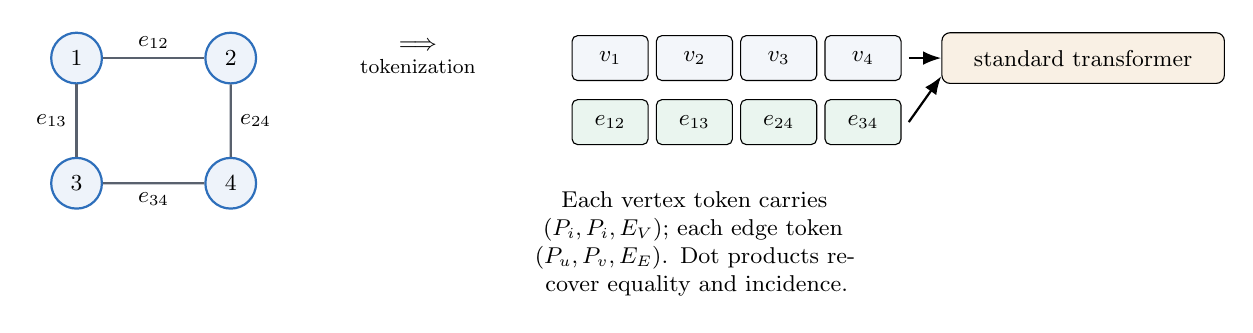
\begin{tikzpicture}[font=\small, node distance=0.85cm, >=Latex, scale=0.92, transform shape]
  \tikzstyle{vtx}=[circle,draw=tokblue,fill=tokblue!8,thick,minimum size=7mm]
  \tikzstyle{edge}=[draw=tokgray,thick]
  \node[vtx] (v1) {$1$};
  \node[vtx, right=1.4cm of v1] (v2) {$2$};
  \node[vtx, below=1cm of v1] (v3) {$3$};
  \node[vtx, right=1.4cm of v3] (v4) {$4$};
  \draw[edge] (v1) -- node[above] {$e_{12}$} (v2);
  \draw[edge] (v1) -- node[left] {$e_{13}$} (v3);
  \draw[edge] (v2) -- node[right] {$e_{24}$} (v4);
  \draw[edge] (v3) -- node[below] {$e_{34}$} (v4);
  \node[right=1.3cm of v2, align=center] (arrow) {$\Longrightarrow$\\[-0.2em]\footnotesize tokenization};
  \node[draw,rounded corners=2pt,fill=toklight,minimum width=1.05cm,minimum height=0.62cm,right=1.2cm of arrow] (t1) {$v_1$};
  \node[draw,rounded corners=2pt,fill=toklight,minimum width=1.05cm,minimum height=0.62cm,right=0.1cm of t1] (t2) {$v_2$};
  \node[draw,rounded corners=2pt,fill=toklight,minimum width=1.05cm,minimum height=0.62cm,right=0.1cm of t2] (t3) {$v_3$};
  \node[draw,rounded corners=2pt,fill=toklight,minimum width=1.05cm,minimum height=0.62cm,right=0.1cm of t3] (t4) {$v_4$};
  \node[draw,rounded corners=2pt,fill=tokgreen!10,minimum width=1.05cm,minimum height=0.62cm,below=0.25cm of t1] (e1) {$e_{12}$};
  \node[draw,rounded corners=2pt,fill=tokgreen!10,minimum width=1.05cm,minimum height=0.62cm,right=0.1cm of e1] (e2) {$e_{13}$};
  \node[draw,rounded corners=2pt,fill=tokgreen!10,minimum width=1.05cm,minimum height=0.62cm,right=0.1cm of e2] (e3) {$e_{24}$};
  \node[draw,rounded corners=2pt,fill=tokgreen!10,minimum width=1.05cm,minimum height=0.62cm,right=0.1cm of e3] (e4) {$e_{34}$};
  \node[below=0.52cm of e2, align=center, text width=5.4cm] (desc) {Each vertex token carries $(P_i,P_i,E_V)$; each edge token $(P_u,P_v,E_E)$. Dot products recover equality and incidence.};
  \node[draw,rounded corners=3pt,fill=tokamber!12,minimum width=3.9cm,minimum height=0.7cm,right=0.55cm of t4] (tr) {standard transformer};
  \draw[->,thick] ($(t4.east)+(0.1,0)$) -- (tr.west);
  \draw[->,thick] ($(e4.east)+(0.1,0)$) -- ($(tr.west)+(0,-0.25)$);
\end{tikzpicture}
\caption{TokenGT-style graph tokenization, redrawn schematically after Kim et al. \cite{kim2022tokengt}.  The architectural novelty is not a graph-specific attention rule; it is the replacement of a vertex-only sequence by vertex and edge tokens whose identifiers make incidence visible to ordinary dot-product attention.}
\label{fig:tokengt}
\end{figure}

\section{Source Map and Preliminaries}

This section fixes notation and summarizes the source results used later.  The purpose is not to reproduce the cited papers, but to expose the exact assumptions that enter the new theorems.

\subsection{Graphs, tensors, and symmetry}

Let $[n]=\{1,\dots,n\}$ and let $\Sn$ act on $[n]$ by relabeling.  A dense order-$k$ hypergraph feature tensor is an element
\[
  X\in \R^{[n]^k\times d}.
\]
For $\pi\in \Sn$, the action is
\[
  (\pi\cdot X)_{i_1,\dots,i_k}
  =X_{\pi^{-1}(i_1),\dots,\pi^{-1}(i_k)}.
\]
A map $F:\R^{[n]^k\times d}\to \R^{[n]^\ell\times d'}$ is permutation equivariant if
\[
  F(\pi\cdot X)=\pi\cdot F(X)
\]
for all $\pi\in\Sn$, where the action on the output is entrywise on $\ell$ indices.  It is invariant if the output is unchanged.

Sparse graphs will be denoted $G=(V,E,X_V,X_E)$, with $|V|=n$, $|E|=m$, vertex features $X_V\in \R^{n\times d_V}$, and edge features $X_E\in \R^{m\times d_E}$.  The sparse and dense views are related by filling a dense order-$2$ tensor with a distinguished null edge feature for missing edges.  The dense view is more convenient for equivariant proofs; the sparse view is more faithful to TokenGT's implementation and to the tropical token-count effect.

\begin{definition}[Graph-to-graph map]
For fixed $n$, an \emph{order-$(k,\ell)$ graph-to-graph map} is a function
\[
  F:\cX_{n,k}\subset \R^{[n]^k\times d}\longrightarrow \R^{[n]^\ell\times d'}.
\]
It is an unlabeled graph-to-graph map only when it is permutation equivariant.  A non-equivariant map on unlabeled graphs is not well-defined: two relabelings of the same graph would demand incompatible outputs.
\end{definition}

\begin{remark}[Why fixed $n$ appears]
Universal approximation is a compact-domain statement.  For graphs of unbounded order, one either studies a family of approximators $\{F_n\}_{n\ge 1}$, one per $n$, or imposes an additional uniformity condition.  Circuit-complexity results below are stated as nonuniform or uniform families accordingly.  The tropical region-counting results are asymptotic in token count, but the network architecture for a fixed maximum size still has a finite input dimension.
\end{remark}

\subsection{TokenGT embeddings}

TokenGT \cite{kim2022tokengt} augments tokens by orthonormal node identifiers and type identifiers.  In dense order-$k$ form, choose an orthonormal matrix $P\in \R^{n\times d_p}$ with rows $P_1,\dots,P_n$ and a type matrix
\[
  E\in \R^{\bell(k)\times d_e},
\]
one row for each equality pattern, or equivalently each equivalence class $\gamma\in [n]^k/\!\sim$ under coordinate equality.  The token for multi-index $i=(i_1,\dots,i_k)$ is
\[
  \mathrm{Tok}_k(X)_i
  =
  \bigl[
    X_i,\,
    P_{i_1},\dots,P_{i_k},\,
    E_{\gamma(i)}
  \bigr].
\]
For ordinary sparse graphs, vertices are treated as diagonal order-$2$ tokens $(i,i)$ and edges as off-diagonal tokens $(u,v)$, matching the practical construction in \cite{kim2022tokengt}.

The key algebraic fact is that the dot products of the identifier coordinates implement equality tests:
\[
  \langle P_a,P_b\rangle = \one\{a=b\}.
\]
Thus attention scores can test whether two token indices share endpoints, whether a token is diagonal, and which equality pattern holds among several indices.

\subsection{Equivariant basis tensors and invariant graph networks}

Invariant and equivariant graph networks (IGNs) \cite{maron2019invariant,maron2019provably,maron2019universality} are built from the full vector space of linear maps commuting with the $\Sn$ action.  For $k,\ell\ge 0$, an equivariant linear layer $L_{k\to \ell}$ has the form
\begin{equation}
  (L_{k\to \ell}X)_i
  =
  \sum_{\mu}\sum_{j\in [n]^k} B^\mu_{i,j}X_jW_\mu
  +
  \sum_\lambda C^\lambda_i b_\lambda ,
  \label{eq:equivlayer}
\end{equation}
where $i\in [n]^\ell$, $\mu$ ranges over equality patterns in $[n]^{\ell+k}$, and $\lambda$ over equality patterns in $[n]^\ell$.  The binary tensors $B^\mu$ and $C^\lambda$ form a basis for the equivariant weight and bias spaces.  There are $\bell(\ell+k)$ weight basis tensors and $\bell(\ell)$ bias basis tensors, independent of $n$.

TokenGT's central theorem says that self-attention over the augmented tokens can approximate these basis tensors head by head.  The proof decomposes the test $(i,j)\in\mu$ into equality-pattern tests on $i$, on $j$, and between coordinates of $i$ and $j$; each is implemented by identifier dot products and then sharpened by softmax.  Consequently, a transformer layer with $\bell(2k)$ heads can approximate an order-$k$ equivariant linear layer $L_{k\to k}$, and a stack can approximate a $k$-IGN \cite{kim2022tokengt}.

\subsection{Universal approximation of sequence transformers}

Yun et al. \cite{yun2020universal} prove that transformers are universal approximators of continuous permutation-equivariant sequence-to-sequence functions, and with trainable positional encodings, of arbitrary continuous sequence-to-sequence functions on compact domains.  Their proof has three conceptual steps: approximate a continuous target by a piecewise-constant function on a grid; use self-attention to compute contextual codes that distinguish grid sequences up to the relevant symmetry; use token-wise feed-forward layers to assign desired values.

This paper uses their result in two ways.  First, it supplies an independent route to finite labeled graph interpolation once a graph is injectively tokenized as a sequence.  Second, the contextual-code idea explains why output-slot tokens are enough to move from graph-level outputs to graph-to-graph outputs on a finite domain.

\subsection{Circuit complexity of transformers}

Hahn \cite{hahn2020limitations} proves limitations for hard and soft self-attention on formal languages: fixed-depth, fixed-head self-attention cannot model certain periodic regular languages or hierarchical languages unless depth or number of heads grows with input length.  Merrill, Sabharwal, and Smith \cite{merrill2022saturated} refine the picture by studying saturated attention.  Saturated attention attends uniformly to all maximizers of a score vector; this strictly generalizes unique hard attention and captures a counting primitive.  Their main circuit result is that saturated transformers over floating-point values are contained in nonuniform $\mathsf{TC}^0$, while saturated rational-valued transformers with very powerful internal functions can recognize all languages.

For graph tokenization, the important lesson is not that TokenGT magically escapes all asymptotic circuit bounds.  It is that edge and vertex tokenization changes the Boolean input basis.  A circuit over graph tokens sees adjacency and incidence predicates directly, whereas a naked vertex transformer without structural encodings sees a bag of vertices and must infer graph structure from absent information.

\subsection{Logic of naked graph transformers}

Ahvonen et al. \cite{ahvonen2026logic} characterize the expressive power of graph transformers and GPS networks without positional or structural encodings.  In the real-valued setting, graph transformers correspond, relative to first-order logic, to propositional logic with a global modality; GPS networks correspond to graded modal logic with a global modality.  In the floating-point setting, counting global modalities become expressible through finite-precision phenomena.

These results are deliberately about ``naked'' graph transformers.  TokenGT is outside that naked model because its identifiers are structural encodings.  Our theorems below can be read as describing what is added by those encodings: incidence tests, equivariant basis tensors, threshold-gate simulations over adjacency bits, and a larger tropical token set.

\subsection{Tropical and toric sources}

The tropical semiring is $\maxplus=\R\cup\{-\infty\}$ with
\[
  a\tropadd b=\max\{a,b\},
  \qquad
  a\tropmul b=a+b.
\]
Tropical polynomials are maxima of affine forms, and their Newton polytopes and normal fans control their linear regions \cite{maclagan2015tropical,zhang2018tropical}.  Su and Liu \cite{su2026tropicalexpressivity} apply Maslov dequantization to attention.  With fixed keys $k_1,\dots,k_N$, the zero-temperature routing partition of query space is a power diagram, and multi-head attention refines normal fans through Minkowski sums.  Hashemi et al. \cite{hashemi2025tropicalattention} and Alpay and Senturk \cite{alpay2026geometry} develop complementary tropical-attention and tropical-circuit perspectives.

Fu \cite{fu2025toricrelu} connects unbiased rational ReLU networks to toric geometry.  Such a network defines a ReLU fan, a toric variety $X_\Sigma$, and a ReLU Cartier divisor whose support function is the output CPWL function up to affine shift.  For tropical polynomials, the toric polytope associated with the divisor agrees with the Newton polytope up to sign.  This gives a powerful bridge, but only under hypotheses that transformers usually violate.

\subsection{Detailed synthesis of the attached papers}
\label{subsec:attached-synthesis}

The five attached papers play different roles in the present theory.  This subsection records the reading synthesis explicitly, because the extension developed here depends as much on their assumptions as on their headline theorems.

\paragraph{Su--Liu: tropical expressivity of transformers.}
The paper \cite{su2026tropicalexpressivity} is the geometric backbone of this work.  Its central move is to place dot-product attention in the log-domain and to analyze the $\tau\to 0$ Maslov limit.  In that limit, the log-sum-exp denominator becomes the tropical polynomial $\max_j\langle q,k_j\rangle$, and the query space is cut into cells by the winning key.  The important technical refinement is the power-diagram interpretation: dot-product maximization is equivalent to weighted nearest-site comparison with weight $\|k_j\|^2$.  This removes a common overcounting error.  Pairwise comparisons among all keys might suggest $O(N^2)$ hyperplanes per head, but only the top-cell structure matters, so a single head has at most $N$ full-dimensional cells.  Multi-head attention then corresponds to common refinement of head fans, or equivalently to the normal fan of a Minkowski sum of head Newton polytopes.  The present paper imports exactly that mechanism and replaces the sequence length $N$ by the TokenGT graph-token count $N_G$.  It also imports the finite-temperature stability estimates, but with the caveat that their prefactor depends on $N_G$.

\paragraph{Yun et al.: sequence-to-sequence universal approximation.}
Yun et al. \cite{yun2020universal} supply the functional-analysis side.  The key idea for this paper is not only their final universal approximation theorem, but the proof architecture: quantize a compact domain, use attention to assign contextual codes that distinguish grid sequences, and then use token-wise feed-forward layers as a lookup mechanism.  This proof explains why a finite graph-to-graph interpolation theorem should use output-slot tokens.  Once a graph is tokenized injectively, a transformer can distinguish finitely many tokenized graphs and assign arbitrary outputs on those finitely many cases.  However, the original theorem is a sequence theorem, and its positional-encoding version is not automatically invariant under graph relabeling.  The present paper therefore separates labeled finite interpolation from unlabeled equivariant approximation.

\paragraph{Kim et al.: TokenGT.}
TokenGT \cite{kim2022tokengt} is the architectural and algebraic source.  Its theorem is stronger than the informal claim that ``edges are tokens.''  The proof shows that orthonormal node identifiers and type identifiers let attention heads approximate every equality-pattern basis tensor in the space of permutation-equivariant linear maps.  For graphs, $k=2$ and there are $\bell(4)=15$ weight bases.  For order-$k$ hypergraphs, $\bell(2k)$ heads suffice to cover the basis tensors.  This paper uses that result twice: first to prove continuous graph-to-graph universality through $k$-IGN universality, and second to interpret equality-pattern attention supports as incidence fans in the tropical skeleton.

\paragraph{Liu et al.: GraphCG and graph-to-graph editing context.}
The GraphCG paper \cite{liu2024graphcg} is not a toric-ReLU paper; its role is contextual.  It studies graph controllable generation and editing in the latent spaces of graph deep generative models, with molecular graphs and point-cloud graphs as primary examples.  Its relevance here is that graph-to-graph maps are not only node-classification or graph-classification abstractions.  In molecular editing, one wants maps that change edge and vertex structure while preserving or steering semantic factors such as functional groups.  This motivates treating graph-to-graph outputs as first-class objects with output slots.  It also illustrates why equivariance matters: the edited molecule should not depend on an arbitrary indexing of atoms, while a labeled internal representation may still be useful for computation.

\paragraph{Hashemi et al.: Tropical Attention.}
Tropical Attention \cite{hashemi2025tropicalattention} provides the algorithmic-reasoning counterpart to Su--Liu's spatial-partition theory.  Its max-plus attention mechanism preserves polyhedral decision structures and simulates tropical circuits and transitive closure.  The present paper does not replace standard attention with their tropical attention layer; instead, it uses their circuit perspective to explain why TokenGT edge tokens are natural carriers for max-plus dynamic programs.  If edge tokens store weights and endpoint identifiers, a zero-temperature graph-token transformer can implement Bellman--Ford-style relaxations by moving information from source vertices to edge tokens and then to target vertices.

\begin{remark}[Assumption ledger]
The following assumptions are used repeatedly.  Functional universality uses fixed graph size and compact feature domains.  Finite interpolation uses a finite graph set and is nonuniform unless a size-uniform resource rule is supplied.  Circuit simulation uses nonuniform polynomial resources unless explicitly stated otherwise.  Tropical region bounds are conditioned on fixed keys or fixed projected context and use zero-temperature CPWL skeletons.  Toric conclusions require rational polyhedral fans and unbiased ReLU support functions, or a homogenized substitute.  Dropping any one of these assumptions changes the theorem.
\end{remark}

\section{TokenGT Graph-to-Graph Universality}
\label{sec:universality}

We now prove the main approximation results.  The section is organized around three increasingly broad senses of ``arbitrary graph-to-graph function.''

First, for unlabeled graphs and continuous features, arbitrary must mean permutation equivariant.  TokenGT is universal for these maps.  Second, for finite graph sets, any isomorphism-respecting function can be exactly interpolated.  Third, if labels are fixed and non-equivariance is allowed, TokenGT plus absolute label identifiers can interpolate arbitrary labeled graph-to-graph maps.  These distinctions are essential.

\subsection{Equivariant universal approximation}

\begin{assumption}[Compact graph-feature domain]
Fix $n,k,\ell,d,d'$ and let $\cX\subset \R^{[n]^k\times d}$ be compact and invariant under $\Sn$.  We consider continuous maps
\[
  F:\cX\to \R^{[n]^\ell\times d'}
\]
with respect to any Euclidean norm.
\end{assumption}

The following theorem is the natural graph-to-graph extension of TokenGT's graph-level theorem.

\begin{theorem}[TokenGT universality for equivariant graph-to-graph maps]
\label{thm:eq-univ}
Let $F:\cX\to \R^{[n]^k\times d'}$ be continuous and permutation equivariant.  For every $\eps>0$, there exists a TokenGT-style transformer operating on order-$k$ tokens with node identifiers and type identifiers such that its first $d'$ output channels define a map $\widehat F$ satisfying
\[
  \sup_{X\in \cX}\|F(X)-\widehat F(X)\|<\eps .
\]
More generally, for output order $\ell$, the same claim holds after adjoining output-slot tokens indexed by $[n]^\ell$ and using cross-slot attention, or equivalently by using a final TokenGT layer approximating $L_{k\to \ell}$.
\end{theorem}

\begin{proof}
We give the proof for $\ell=k$ first.  By the universality theorem for invariant/equivariant graph networks \cite{maron2019universality,keriven2019universal}, continuous $\Sn$-equivariant maps on compact order-$k$ tensor domains can be uniformly approximated by networks formed from equivariant linear layers of the form \eqref{eq:equivlayer}, pointwise nonlinearities, and a final equivariant readout.  Thus, for $\eps>0$, there exists a $k$-IGN $G$ such that
\[
  \sup_{X\in\cX}\|F(X)-G(X)\|<\eps/2.
\]

It remains to approximate $G$ by a TokenGT transformer.  Each equivariant linear layer in $G$ is a finite sum over basis tensors $B^\mu$ and $C^\lambda$.  TokenGT's identifier construction supplies, for every equality pattern $\mu\in [n]^{2k}/\!\sim$, an attention head whose attention matrix approximates the row-normalized basis tensor $B^\mu$ to arbitrary precision.  The normalizing row sums depend only on the equality class of the query multi-index; the type identifier $E_{\gamma(i)}$ allows a token-wise MLP to recover and undo these factors.  The same MLP inserts the bias basis $C^\lambda$.  Therefore, a transformer block with $\bell(2k)$ heads and a sufficiently wide feed-forward layer approximates any chosen equivariant linear layer $L_{k\to k}$ uniformly on $\cX$.

Pointwise nonlinearities are token-wise and hence are directly implemented by the feed-forward subnet.  Composing these approximations layer by layer gives a TokenGT transformer $\widehat G$ with
\[
  \sup_{X\in\cX}\|G(X)-\widehat G(X)\|<\eps/2
\]
after choosing sufficiently accurate head sharpness and MLP approximations.  The triangle inequality proves the claim.

For $\ell\ne k$, append output-slot tokens labeled by multi-indices $i\in[n]^\ell$ with identifiers $(P_{i_1},\dots,P_{i_\ell},E_{\gamma(i)})$.  The same equality-pattern scoring argument approximates $B^\mu\in \R^{[n]^\ell\times [n]^k}$ for $\mu\in [n]^{\ell+k}/\!\sim$, hence approximates $L_{k\to\ell}$.  This supplies the final equivariant readout.  Alternatively, one may use a dense order-$\max\{k,\ell\}$ representation and project to the desired output slots.  Both constructions preserve equivariance because the identifiers transform consistently under $\Sn$.
\end{proof}

\begin{remark}[Why this is stronger than a node-only graph transformer]
A node-only transformer with no structural encoding is permutation equivariant over the multiset of node features, but it cannot distinguish two graphs with identical node features and different edge sets.  TokenGT's edge tokens make the edge relation part of the sequence and its identifiers make incidence accessible to attention.  The universality theorem therefore applies to graph functions depending on adjacency, cycles, substructures, and edge labels.
\end{remark}

\begin{corollary}[Universal approximation for ordinary graph-to-graph maps]
\label{cor:ordinary}
Let $\cX$ be a compact set of graphs on $n$ vertices represented by dense adjacency/edge-feature tensors $X\in\R^{[n]^2\times d}$.  Every continuous permutation-equivariant node-and-edge output map
\[
  F:\cX\to \R^{[n]^2\times d'}
\]
can be uniformly approximated by a TokenGT transformer with vertex and edge tokens.
\end{corollary}

\begin{proof}
Apply \Cref{thm:eq-univ} with $k=\ell=2$.  Vertex outputs are the diagonal slots $(i,i)$ and edge outputs are the off-diagonal slots $(i,j)$, with missing edges represented by the null edge feature if a sparse graph is embedded densely.
\end{proof}

\subsection{Finite graph-to-graph interpolation}

Continuous universal approximation is not the only relevant sense of expressivity.  Graph algorithms and Boolean graph properties often live on finite domains.  In that setting, exact interpolation is possible under weaker analytic assumptions.

\begin{definition}[Finite graph domain]
Let $\cD$ be a finite set of graphs on at most $n$ vertices, with vertex and edge attributes in finite alphabets.  A graph-to-graph function $F:\cD\to\cD'$ is \emph{isomorphism respecting} if $G\cong G'$ implies $F(G)\cong F(G')$, with output relabeling induced by input relabeling when vertex identities are preserved.
\end{definition}

\begin{theorem}[Exact finite interpolation on graph tokens]
\label{thm:finite-interp}
Fix a finite labeled graph domain $\cD$ with a maximum of $n$ vertices and $m_{\max}$ edges.  Encode each graph by TokenGT vertex and edge tokens, padded to a fixed length, and add output-slot tokens for every possible output vertex and edge slot.  For every function $F:\cD\to\cY$ into a finite graph-output alphabet, there exists a finite-depth transformer with TokenGT identifiers whose output equals $F(G)$ on every $G\in\cD$.

If the graphs are unlabeled, the same statement holds exactly for isomorphism-respecting $F$ after quotienting by relabeling; non-equivariant functions are impossible on unlabeled graphs.
\end{theorem}

\begin{proof}
Because $\cD$ is finite, it suffices to construct an injective code $c(G)$ for each input graph and then implement a lookup table.  TokenGT tokenization is injective on labeled graphs: vertex tokens contain labels and vertex identifiers, edge tokens contain endpoint identifiers and edge labels, and padding uses a distinguished type.  Hence two distinct labeled graphs produce distinct multisets of augmented tokens.

A transformer can compute a contextual code that distinguishes finitely many token sequences.  One route is to invoke the finite-grid contextual mapping construction of Yun et al. \cite{yun2020universal}: since the tokenized inputs form a finite subset of Euclidean sequence space, self-attention layers can map each sequence to a unique contextual scalar on a graph token or on every output slot.  A simpler nonuniform construction is to assign one attention/MLP test per graph in $\cD$: identifier dot products test the presence of each required vertex and edge token, and feed-forward threshold units combine these tests into an indicator $\one\{G=G_0\}$.  Since $\cD$ is finite, only finitely many such indicators are needed.

After these indicators are available, a token-wise feed-forward lookup table assigns to each output slot the corresponding symbol of $F(G)$.  ReLU networks exactly interpolate finite sets by separating points with small polyhedral neighborhoods; equivalently, a sufficiently wide MLP implements the finite table.  The transformer output therefore equals $F(G)$ on $\cD$.

For unlabeled graphs, if $G$ and $\pi G$ represent the same input, any well-defined output must satisfy $F(\pi G)=\pi F(G)$.  The above construction can be symmetrized over each orbit by using canonical orbit indicators or by applying the equivariant construction in \Cref{thm:eq-univ} to one-hot finite features.  A non-equivariant target would assign two different outputs to the same unlabeled object, so no graph model respecting unlabeled semantics can realize it.
\end{proof}

\begin{remark}[Output slots are part of the representation]
Graph-to-graph functions require a place to write the output.  Sequence-to-sequence transformers use output positions; image transformers use patches; TokenGT can use vertex and edge output slots.  Without output slots, a graph-level token can represent a graph, but an additional decoder is needed to expand that representation back into node and edge outputs.
\end{remark}

\subsection{A limitation: variable-size uniformity}

The preceding theorems are fixed-size or nonuniform.  This is unavoidable without further assumptions.

\begin{proposition}[No size-uniform universality without a resource growth rule]
\label{prop:no-uniform}
There is no single finite transformer with fixed embedding dimension, fixed number of layers, and fixed number of heads that exactly realizes every isomorphism-respecting Boolean graph property on graphs of all sizes.
\end{proposition}

\begin{proof}
A fixed finite transformer has a fixed computation graph applied uniformly to all sequence lengths.  Over finite precision, its recognized languages are contained in some uniform or nonuniform circuit class determined by the attention model; for saturated floating-point transformers, the relevant nonuniform upper bound is $\mathsf{TC}^0$ \cite{merrill2022saturated}.  There exist decidable graph properties outside any fixed constant-depth polynomial-size threshold-circuit family, for example by standard counting and hierarchy arguments in circuit complexity.  Therefore a fixed transformer cannot realize all graph properties on all sizes.  Over real numbers without precision restrictions, one can encode unbounded information in a real parameter, but that is a non-effective model and not a uniform approximation theorem.  Thus any honest variable-size universality statement must specify how depth, width, heads, precision, or external computation grows with $n$.
\end{proof}

\section{Boolean Circuits on Graph Tokens}
\label{sec:circuits}

The Boolean-circuit perspective complements the continuous approximation theorem.  It asks how graph tokenization changes the Boolean primitives available to attention.  The answer is concise: TokenGT turns graph relations into tokens and identifier dot products; saturated or sharply approximated soft attention turns selected token sets into threshold-gate inputs.

\subsection{Graph-token circuits}

Let a graph on $n$ vertices be represented by Boolean variables:
\[
  a_{uv}\in\{0,1\}\quad (u,v\in[n]),
  \qquad
  x_{u,r}\in\{0,1\},
  \qquad
  e_{uv,s}\in\{0,1\},
\]
encoding adjacency, vertex labels, and edge labels.  A nonuniform graph circuit family $\{C_n\}$ has one Boolean circuit for each $n$.  A $\mathsf{TC}^0$ graph circuit family has polynomial size, constant depth, and unbounded fan-in threshold gates.

\begin{definition}[TokenGT circuit simulation]
A TokenGT circuit simulation of $\{C_n\}$ consists, for each $n$, of a TokenGT transformer whose sequence contains input graph tokens, gate tokens for each gate of $C_n$, and output tokens.  The simulation is correct if each gate token stores the gate value after the corresponding layer and output tokens store $C_n$'s outputs.
\end{definition}

\begin{figure}[t]
\centering
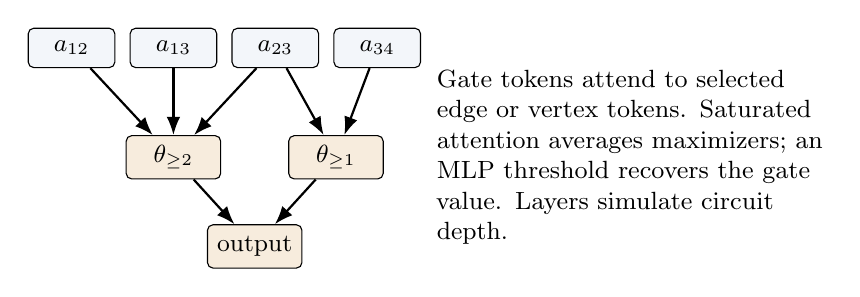
\begin{tikzpicture}[font=\small, >=Latex, node distance=0.65cm]
  \tikzstyle{tok}=[draw,rounded corners=2pt,fill=toklight,minimum width=1.1cm,minimum height=0.5cm]
  \tikzstyle{gate}=[draw,rounded corners=2pt,fill=tokamber!15,minimum width=1.2cm,minimum height=0.55cm]
  \node[tok] (a12) {$a_{12}$};
  \node[tok,right=0.18cm of a12] (a13) {$a_{13}$};
  \node[tok,right=0.18cm of a13] (a23) {$a_{23}$};
  \node[tok,right=0.18cm of a23] (a34) {$a_{34}$};
  \node[gate,below=0.85cm of a13] (g1) {$\theta_{\ge 2}$};
  \node[gate,right=0.85cm of g1] (g2) {$\theta_{\ge 1}$};
  \node[gate,below=0.85cm of $(g1)!0.5!(g2)$] (out) {output};
  \draw[->,thick] (a12) -- (g1);
  \draw[->,thick] (a13) -- (g1);
  \draw[->,thick] (a23) -- (g1);
  \draw[->,thick] (a23) -- (g2);
  \draw[->,thick] (a34) -- (g2);
  \draw[->,thick] (g1) -- (out);
  \draw[->,thick] (g2) -- (out);
  \node[right=0.55cm of g2, text width=4.9cm, align=left] {Gate tokens attend to selected edge or vertex tokens. Saturated attention averages maximizers; an MLP threshold recovers the gate value. Layers simulate circuit depth.};
\end{tikzpicture}
\caption{Circuit simulation over graph tokens.  This is a schematic adaptation of the saturated-transformer threshold-circuit viewpoint of Merrill et al. \cite{merrill2022saturated} to TokenGT's edge/vertex token basis.}
\label{fig:circuit}
\end{figure}

\begin{theorem}[TokenGT simulates nonuniform threshold circuits]
\label{thm:tc0-sim}
Let $\{C_n\}$ be a nonuniform $\mathsf{TC}^0$ circuit family over adjacency, vertex-label, and edge-label bits, with depth $D$ and polynomial size $S(n)$.  There is a nonuniform family of TokenGT transformers with $D+O(1)$ layers and polynomially many tokens, heads, and hidden units that computes the same graph-to-graph Boolean function.  The construction uses vertex tokens, edge tokens, gate tokens, and output-slot tokens.
\end{theorem}

\begin{proof}
Fix $n$ and a circuit $C_n$.  Create one input token for each vertex and edge bit and one gate token for each internal gate.  Gate tokens are given identifiers encoding the gate's layer and its incoming-wire set.  Because the construction is nonuniform, these identifiers may depend on $C_n$.

Suppose all gate values at depth $r$ are already stored in their gate tokens.  For a threshold gate $g$ at depth $r+1$, choose an attention head whose score is maximal exactly on the tokens feeding into $g$.  This selection can be implemented by dot products between the gate identifier and source identifiers, just as TokenGT uses identifier dot products to test incidence.  Under saturated attention, the head returns the average of the selected source values.  A token-wise MLP compares this average with the threshold divided by the fan-in, thereby computing the threshold gate.  AND, OR, and NOT are special cases or are implemented by the MLP.

All gates of the same circuit depth can be computed in parallel because each has its own gate token, and polynomially many heads or hidden channels are allowed in the nonuniform family.  Repeating for $D$ circuit depths stores all output gate values, which are copied into output-slot tokens.  This simulates $C_n$ with constant depth $D+O(1)$ and polynomial resources.
\end{proof}

\begin{corollary}[Majority, parity, and subgraph-count thresholds]
For fixed graph size $n$, TokenGT transformer families of the kind in \Cref{thm:tc0-sim} compute majority over edges, parity over edges, and any constant-depth threshold combination of fixed subgraph-count predicates that has polynomial-size threshold circuits.
\end{corollary}

\begin{proof}
Majority and parity are in nonuniform $\mathsf{TC}^0$.  Fixed subgraph-count thresholds can be expressed by polynomially many conjunctions over edge variables followed by threshold gates when the pattern size is fixed.  Apply \Cref{thm:tc0-sim}.
\end{proof}

\subsection{Relation to Hahn and Merrill--Sabharwal--Smith}

Hahn's limitation theorem \cite{hahn2020limitations} applies to fixed-depth, fixed-head self-attention models on unbounded sequences and shows failures on periodic and hierarchical formal languages.  Merrill et al. \cite{merrill2022saturated} show that saturated attention over floats is more powerful than unique hard attention but remains inside $\mathsf{TC}^0$.  The graph-token theorem above is consistent with both.  It is nonuniform in $n$, and it uses polynomially many gate tokens and channels to simulate a polynomial-size circuit.  It does not claim that a single fixed TokenGT solves parity for all graph sizes without resource growth.

\begin{proposition}[Hard-attention edge case]
\label{prop:hard-edge}
If each graph-token attention head is restricted to unique hard attention and the number of layers and heads is fixed independently of $n$, then TokenGT cannot in general compute all $\mathsf{TC}^0$ graph properties uniformly over $n$.
\end{proposition}

\begin{proof}
Unique hard attention selects one maximizer rather than averaging all maximizers.  It therefore lacks the direct counting primitive used in \Cref{thm:tc0-sim}.  On word-shaped graphs, TokenGT with only successor edges contains ordinary hard-attention transformers as a special case.  Hahn-style reductions then rule out periodic languages such as parity under fixed-depth and fixed-head assumptions.  Since parity of a word-shaped graph's edge or vertex labels is a graph property, the claimed uniform computation of all $\mathsf{TC}^0$ graph properties would contradict those lower bounds.
\end{proof}

\subsection{Why structural tokenization matters for graph logic}

The logic characterizations of naked graph transformers \cite{ahvonen2026logic} show that, without positional or structural encodings, pure graph transformers are essentially global bag-of-vertices models.  They can express global existence and, over floats, certain bounded counting modalities, but they do not have direct access to adjacency.  TokenGT changes the underlying structure by adding edge tokens and incidence identifiers.  In logical terms, it expands the vocabulary seen by the transformer from unary vertex predicates to a token structure with endpoint relations.

\begin{proposition}[Separation from naked graph transformers]
\label{prop:naked-separation}
There exist pairs of graphs $G,H$ with identical multisets of vertex labels but different edge sets such that a naked graph transformer without structural encodings assigns identical vertex representations to $G$ and $H$, while a TokenGT transformer distinguishes them in one attention layer.
\end{proposition}

\begin{proof}
Let $G$ and $H$ have the same $n$ vertices and identical vertex features, but let $G$ contain an edge $(1,2)$ absent from $H$.  A naked graph transformer whose input is only the multiset of vertex features receives identical token multisets for $G$ and $H$, so by permutation equivariance it computes identical multisets of representations.

TokenGT includes an edge token for $(1,2)$ in $G$ and not in $H$ (or includes a dense edge token with a different edge-present bit).  The vertex token for $1$ has identifiers $(P_1,P_1)$ and the edge token for $(1,2)$ has identifiers $(P_1,P_2)$.  Their dot product in the identifier coordinates detects incidence.  An attention head can attend from a graph token to edge-present tokens incident to vertex $1$, and an MLP can threshold whether such a token exists.  Thus $G$ and $H$ are distinguished.
\end{proof}

\section{Tropical Geometry of Tokenized Graph Attention}
\label{sec:tropical}

We now transfer the tropical expressivity theory from sequences to TokenGT.  The key point is that the tropical skeleton depends on the token set.  TokenGT replaces the node-token set by a graph-token set that includes edges and, in order-$k$ form, hyperedges or all $k$-tuples.

\subsection{Power diagrams for graph tokens}

For a fixed set of graph tokens $t_1,\dots,t_{N_G}$, let their projected keys be $k_1,\dots,k_{N_G}\in \R^d$.  A query $q\in \R^d$ has logits
\[
  s_j(q)=\langle q,k_j\rangle .
\]
In the zero-temperature limit, attention selects $\argmax_j s_j(q)$.  As in \cite{su2026tropicalexpressivity}, this is equivalent to a power diagram:
\[
  \langle q,k_j\rangle \ge \langle q,k_\ell\rangle
  \quad\Longleftrightarrow\quad
  \|q-k_j\|^2-\|k_j\|^2
  \le
  \|q-k_\ell\|^2-\|k_\ell\|^2.
\]
Thus the sites are the graph-token keys and the weights are $\|k_j\|^2$.

\begin{figure}[t]
\centering
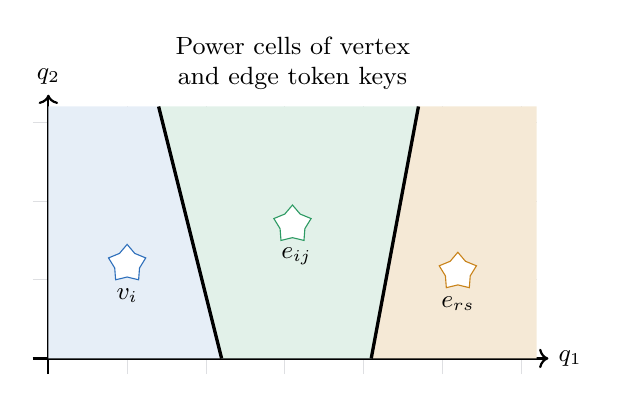
\begin{tikzpicture}[font=\small, scale=1.0]
  \draw[step=1cm, tokgray!20, very thin] (-0.2,-0.2) grid (6.2,3.2);
  \draw[thick,->] (-0.2,0) -- (6.35,0) node[right] {$q_1$};
  \draw[thick,->] (0,-0.2) -- (0,3.35) node[above] {$q_2$};
  \fill[tokblue!12] (0,0) -- (2.2,0) -- (1.4,3.2) -- (0,3.2) -- cycle;
  \fill[tokgreen!14] (2.2,0) -- (4.1,0) -- (4.7,3.2) -- (1.4,3.2) -- cycle;
  \fill[tokamber!18] (4.1,0) -- (6.2,0) -- (6.2,3.2) -- (4.7,3.2) -- cycle;
  \draw[very thick] (2.2,0) -- (1.4,3.2);
  \draw[very thick] (4.1,0) -- (4.7,3.2);
  \node[star,star points=5,draw=tokblue,fill=white,minimum size=5pt] at (1.0,1.2) {};
  \node[star,star points=5,draw=tokgreen,fill=white,minimum size=5pt] at (3.1,1.7) {};
  \node[star,star points=5,draw=tokamber,fill=white,minimum size=5pt] at (5.2,1.1) {};
  \node at (1.0,0.8) {$v_i$};
  \node at (3.15,1.3) {$e_{ij}$};
  \node at (5.2,0.7) {$e_{rs}$};
  \node[align=center,text width=5.2cm] at (3.1,3.75) {Power cells of vertex and edge token keys};
\end{tikzpicture}
\caption{A conditioned query-space partition for graph tokens.  This figure is an original schematic based on the power-diagram analysis of Su and Liu \cite{su2026tropicalexpressivity}; TokenGT changes the sites from ordinary sequence tokens to vertex and edge tokens.}
\label{fig:power}
\end{figure}

\begin{definition}[Graph-token count]
For a sparse graph $G=(V,E)$, define $N_G=|V|+|E|+c$, where $c$ counts optional special tokens such as a graph token or output slots.  For dense order-$k$ tokenization, define $N_{n,k}=n^k+c$.
\end{definition}

\begin{proposition}[Single-head graph-token polytope]
\label{prop:single-head}
In conditioned zero-temperature TokenGT attention with $N_G$ graph tokens and fixed projected keys in $\R^d$, the single-head routing potential has Newton polytope
\[
  P=\conv\{k_1,\dots,k_{N_G}\}.
\]
Hence the number of full-dimensional power cells is at most $N_G$, and at most the number of vertices of $P$ if some token keys are non-extreme or have empty cells.
\end{proposition}

\begin{proof}
The tropical denominator is
\[
  P_{\mathrm{den}}(q)=\max_{1\le j\le N_G}\langle q,k_j\rangle.
\]
Its Newton polytope is the convex hull of the exponent/slope vectors $k_j$.  The normal fan of $P$ gives the domains on which a particular key is maximizer.  Non-extreme keys do not define full-dimensional normal cones, and power weights can make cells empty.  Thus the number of full-dimensional cells is bounded by $\#\Vtx(P)\le N_G$.
\end{proof}

\subsection{Multi-head graph-token complexity}

Let $P_h=\conv\{k^{(h)}_1,\dots,k^{(h)}_{N_G}\}$ be the head polytope of head $h$.  Multi-head aggregation induces the common refinement of normal fans, equivalently the normal fan of the Minkowski sum
\[
  P_{\mathrm{MHSA}}=P_1+\cdots+P_H.
\]

\begin{theorem}[Graph-token MHSA polytope bound]
\label{thm:mhsa-graph}
Fix dimension $d$ and number of heads $H$.  For conditioned zero-temperature TokenGT attention with $N_G$ graph tokens, the number $V_{\mathrm{multi}}$ of vertices of the effective multi-head Newton polytope satisfies
\[
  V_{\mathrm{multi}}
  \le
  \begin{cases}
    O(N_G^H), & H\le d,\\
    O((HN_G)^{\lfloor d/2\rfloor}), & H>d.
  \end{cases}
\]
Under generic choices of independent head projections and $H\le d$, there are configurations with $V_{\mathrm{multi}}=\Omega(N_G^H)$.
\end{theorem}

\begin{proof}
The upper bound is the standard Minkowski-sum vertex bound used in tropical attention analysis \cite{gritzmann1993minkowski,su2026tropicalexpressivity}.  When $H\le d$ and summands are in sufficiently general position, mixed vertices of $P_1+\cdots+P_H$ are sums of one vertex from each $P_h$, yielding $O(N_G^H)$ possible mixed vertices and $\Omega(N_G^H)$ realizable vertices for cyclic or neighborly generic configurations.  When $H>d$, the resulting polytope is still $d$-dimensional with at most $HN_G$ generating vertices across summands; McMullen-type upper bounds give $O((HN_G)^{\lfloor d/2\rfloor})$ for fixed $d$.  The normal fan of the Minkowski sum is the common refinement of head fans, so this vertex count bounds the number of full-dimensional refined routing cones.
\end{proof}

\subsection{Depth and graph-token linear regions}

We now state the TokenGT version of the tropical linear-region theorem.  It is conditioned in the same sense as \cite{su2026tropicalexpressivity}: keys are fixed when counting regions in one query embedding, and full-input self-attention requires the caveats in \Cref{sec:toric}.

\begin{theorem}[TokenGT tropical region bound]
\label{thm:tokengt-regions}
Consider a depth-$L$ TokenGT transformer in the zero-temperature tropical skeleton, with graph-token count $N_G$, embedding dimension $d$, feed-forward width $d_{\mathrm{ff}}$, and $H\ge d$ heads.  Assume generic head projections, nonempty power cells, and ReLU feed-forward layers in general position on each attention cell.  Treating $d,H,d_{\mathrm{ff}},L$ as fixed except where displayed, the maximum number of full-dimensional conditioned query-space linear regions satisfies
\[
  \mathcal{N}_{\mathrm{TokenGT}}(N_G,d,L)
  =
  \Theta(N_G^{dL})
\]
up to constants depending on $d,H,d_{\mathrm{ff}}$, and $L$.
\end{theorem}

\begin{proof}
For one layer, \Cref{thm:mhsa-graph} gives $O(N_G^d)$ effective routing cells in the saturated-head regime $H\ge d$, after absorbing dimension-dependent constants.  On each routing cell, zero-temperature attention is affine or piecewise constant in the log-lifted skeleton, and the ReLU feed-forward layer further subdivides by a bounded number of hyperplanes depending on $d_{\mathrm{ff}}$ and $d$, not on $N_G$.  Thus one layer has $O(N_G^d)$ regions.

For depth $L$, composition multiplies the maximal region count, giving the upper bound $O(N_G^{dL})$ under the same recurrence used for CPWL networks.  For the lower bound, place head keys in generic parabolic-lifting configurations so that the power diagram realizes $\Omega(N_G^d)$ cells in the $d$ query coordinates.  Configure the feed-forward block as coordinate-wise sawtooth folds that map each cell affinely onto a common invariant box, with residual connections preserving non-collapse.  Repeating the construction across $L$ layers yields $\Omega(N_G^{dL})$ regions.  This is the graph-token substitution of the constructive lower-bound argument in \cite{su2026tropicalexpressivity}.
\end{proof}

\begin{corollary}[Dense graph scaling]
\label{cor:dense-scaling}
For ordinary dense graphs on $n$ vertices represented by all ordered edge tokens, $N_G=n^2+O(1)$, and hence
\[
  \mathcal{N}_{\mathrm{TokenGT}}=\Theta(n^{2dL})
\]
under the hypotheses of \Cref{thm:tokengt-regions}.  For dense order-$k$ hypergraph tokenization, $N_G=n^k+O(1)$ and
\[
  \mathcal{N}_{\mathrm{TokenGT}}=\Theta(n^{kdL}).
\]
\end{corollary}

\begin{proof}
Substitute $N_G=n^2+O(1)$ or $N_G=n^k+O(1)$ into \Cref{thm:tokengt-regions}.
\end{proof}

\begin{corollary}[Sparse edge case]
\label{cor:sparse-edge}
On graph families with $m=O(n)$, sparse TokenGT has $N_G=n+m+O(1)=O(n)$, so the tropical region exponent in $n$ remains $\Theta(n^{dL})$.  Edge tokenization may still improve constants and expressible relations, but it does not change the asymptotic exponent in $n$.
\end{corollary}

\subsection{Incidence fans}

TokenGT's identifiers introduce a structured subfan before learning.  Equality of identifiers is not learned; it is hard-coded by orthonormality.

\begin{definition}[Incidence score]
For a vertex token $v_w$ and an edge token $e_{uv}$, define the identifier incidence score
\[
  I(w;u,v)=\langle (P_w,P_w),(P_u,P_v)\rangle
  =
  \one\{w=u\}+\one\{w=v\}.
\]
More generally, for order-$k$ tokens, identifier scores are sums of equality indicators among coordinates.
\end{definition}

\begin{proposition}[Identifier-induced basis regions]
\label{prop:incidence-fan}
In TokenGT, every equality-pattern basis tensor $B^\mu$ for an order-$k$ equivariant layer is realizable as a zero-temperature attention support pattern determined solely by identifier coordinates.  Consequently, the tropical routing fan contains refinements corresponding to incidence and equality-pattern tests, independent of input features.
\end{proposition}

\begin{proof}
The proof is the TokenGT basis-tensor construction.  For a target equality pattern $\mu$ over query multi-index $i$ and key multi-index $j$, form a score
\[
  \delta(i,j;\mu)=
  \text{type tests on } i,j
  +
  \sum_{a,b} \sigma_{ab}\one\{i_a=j_b\},
\]
where $\sigma_{ab}=+1$ if equality is required by $\mu$ and $-1$ otherwise, with small margins separating correct and incorrect type classes.  Each equality indicator is an identifier dot product.  Therefore $\delta(i,j;\mu)$ is a dot-product attention score in an expanded identifier coordinate system.  The zero-temperature softmax selects exactly the keys satisfying $(i,j)\in\mu$, up to row normalization.  Hence the support pattern of $B^\mu$ is a tropical attention cell structure independent of $X$.
\end{proof}

\subsection{Finite-temperature stability}

The tropical skeleton is a limit.  At finite temperature $\tau$, the log-sum-exp potential
\[
  P_\tau(s)=\tau\log\sum_{j=1}^{N_G}\exp(s_j/\tau)
\]
is smooth.  On a stable region where one token wins by margin $\delta$, the standard estimates give
\[
  0\le P_\tau(s)-\max_j s_j\le \tau\log(1+(N_G-1)e^{-\delta/\tau}),
\]
\[
  \|\nabla P_\tau(s)-e_i\|_1\le 2(N_G-1)e^{-\delta/\tau},
  \qquad
  \|\nabla^2P_\tau(s)\|_2\le \frac{1}{\tau}(N_G-1)e^{-\delta/\tau}.
\]
The graph-token count appears in the prefactor.  Thus increasing $N_G$ by adding edge tokens increases the number of possible regions, but it also increases the margin required for the same finite-temperature sharpness.  A useful rule of thumb is
\[
  \delta \gtrsim \tau\log N_G
\]
to keep the stability error small.  This is a genuine tradeoff: TokenGT's larger token set expands tropical expressivity, but finite-temperature models must learn margins large enough to make the expanded routing skeleton operational.

\section{Tropical Circuits and Graph Algorithms}

Tropical Attention \cite{hashemi2025tropicalattention} and the tropical-polynomial-circuit view of transformers \cite{alpay2026geometry} emphasize that max-plus operations naturally simulate dynamic programs.  TokenGT adds an explicit graph substrate to this story: edge tokens are the arcs over which path or flow recurrences operate.

\begin{definition}[Max-plus graph dynamic program]
Let $\Gamma=(V,E)$ be a directed graph with weights $w:E\to \R\cup\{-\infty\}$.  A horizon-$T$ max-plus dynamic program updates states
\[
  d_v^{(t+1)}
  =
  \max_{(u,v)\in E}\{d_u^{(t)}+w_{uv}\}.
\]
This includes longest-path recurrences on acyclic graphs and, after sign reversal, shortest-path recurrences.
\end{definition}

\begin{theorem}[TokenGT tropical simulation of edge-local max-plus updates]
\label{thm:maxplus}
Fix a graph size $n$ and horizon $T$.  A TokenGT transformer with edge tokens can simulate $T$ steps of the max-plus update above in $T+O(1)$ zero-temperature attention layers, using vertex tokens to store $d_v^{(t)}$ and edge tokens to store $w_{uv}$ and endpoints.
\end{theorem}

\begin{proof}
At step $t$, each edge token $(u,v)$ attends to the vertex token $u$ using identifier equality between its source endpoint $P_u$ and the vertex identifier.  Its feed-forward block adds the edge weight $w_{uv}$ to the retrieved state $d_u^{(t)}$.  Then each vertex token $v$ attends over incoming edge tokens whose target endpoint equals $P_v$ and takes the tropical maximum of their candidate values.  In zero-temperature attention, this is a max over selected incident edge tokens.  The identifier tests enforce incidence, and the max-plus addition is ordinary addition in the value channel.  Repeating this two-phase edge-to-vertex update simulates the dynamic program.
\end{proof}

\begin{remark}[Comparison with latent token graphs]
Alpay and Senturk \cite{alpay2026geometry} interpret high-confidence attention as Bellman--Ford on a latent complete token graph.  TokenGT makes an external graph available as tokens.  The latent graph still exists, but attention can now be biased or trained to follow the observed edge-token incidence structure.  This is the algorithmic counterpart of the expressivity results above.
\end{remark}

\section{Toric Geometry: Conditional Bridge and Counterexamples}
\label{sec:toric}

The tropical and toric perspectives meet through fan geometry only under explicit structural hypotheses.  Certain transformer skeletons sit naturally in a fan-based tropical--toric dictionary, but general transformers do not.

\subsection{What Fu's toric-ReLU theorem gives}

Fu \cite{fu2025toricrelu} considers unbiased feed-forward ReLU networks with rational weights.  Such a network computes a continuous piecewise-linear function $f:\R^{n_0}\to\R$.  Its linearity domains form a ReLU fan $\Sigma_f$ under appropriate hypotheses; the associated toric variety $X_{\Sigma_f}$ carries a ReLU Cartier divisor $D_f$ whose support function is $f$ up to affine shift.  If $f$ is a tropical polynomial, then the polytope associated with $-D_f$ agrees with $-\Newt(f)$, and line-bundle volumes match Newton-polytope volumes.

This is a theorem about conical rational polyhedral fans and support functions.  It does not apply automatically to arbitrary CPWL complexes with biases, and it does not apply to smooth non-CPWL functions.

\subsection{A conditional transformer bridge}

\begin{assumption}[Toric-compatible transformer skeleton]
\label{ass:toric-compatible}
We say a transformer block is toric-compatible on a domain $\Omega$ if:
\begin{enumerate}
  \item attention is evaluated in the zero-temperature hard-routing limit;
  \item keys are fixed or attention scores are affine functions of the query variables on $\Omega$;
  \item all routing hyperplanes have rational coefficients;
  \item feed-forward subnets are unbiased ReLU networks with rational weights, or are homogenized into such networks;
  \item normalization layers and finite-temperature softmax are omitted; and
  \item value channels are handled in a real CPWL model, not through undefined signed logarithms.
\end{enumerate}
\end{assumption}

\begin{theorem}[Conditional tropical--toric bridge for transformer skeletons]
\label{thm:conditional-toric}
Under \Cref{ass:toric-compatible}, each scalar output channel of a finite-depth transformer skeleton is a rational CPWL function whose linearity domains refine a rational polyhedral fan after homogenization.  If the scalar channel is convex, equivalently a tropical polynomial after affine shift, then its Newton polytope agrees up to sign with the polytope of the associated toric Cartier divisor on the fan.  Thus the skeleton lies in the intersection of tropical and toric geometry in the precise sense of support functions on rational fans.
\end{theorem}

\begin{proof}
Zero-temperature fixed-key attention selects maxima of finitely many rational affine forms.  Therefore each scalar routing potential is a tropical polynomial, and each selected value channel is CPWL after composing with rational ReLU feed-forward maps.  Finite compositions and sums of CPWL functions are CPWL.  With rational coefficients, the domains of linearity form a rational polyhedral complex.  Homogenizing affine coordinates converts this complex into a conical fan in one higher dimension when the usual compatibility conditions hold.

On that fan, the scalar CPWL function is a support function.  Fu's toric-ReLU dictionary then associates a toric variety and a Cartier or $\Q$-Cartier divisor.  When the scalar channel is convex, it is a tropical polynomial after affine shift, and Fu's theorem identifies the divisor polytope $P_{-D}$ with $-\Newt(f)$ and the corresponding volumes.  This proves the conditional bridge.
\end{proof}

\begin{figure}[t]
\centering
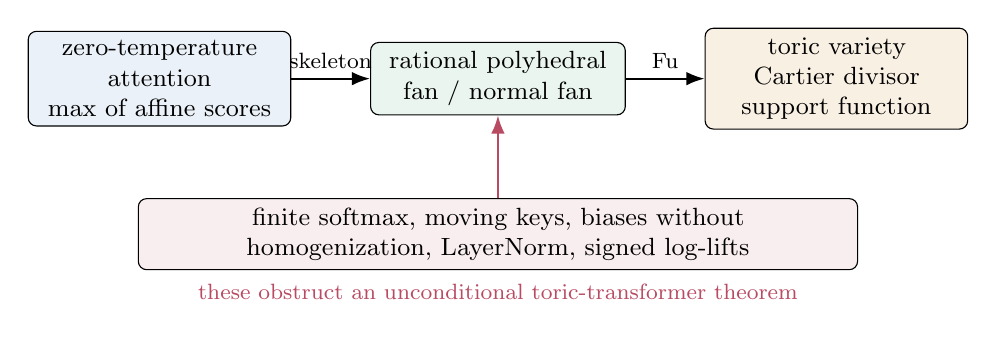
\begin{tikzpicture}[font=\small, >=Latex, node distance=0.85cm]
  \node[draw,rounded corners=3pt,fill=tokblue!10,text width=3.1cm,align=center] (trop) {zero-temperature\\attention\\max of affine scores};
  \node[draw,rounded corners=3pt,fill=tokgreen!10,text width=3.0cm,align=center,right=1.0cm of trop] (fan) {rational polyhedral\\fan / normal fan};
  \node[draw,rounded corners=3pt,fill=tokamber!12,text width=3.1cm,align=center,right=1.0cm of fan] (toric) {toric variety\\Cartier divisor\\support function};
  \draw[->,thick] (trop) -- (fan) node[midway,above] {\footnotesize skeleton};
  \draw[->,thick] (fan) -- (toric) node[midway,above] {\footnotesize Fu};
  \node[draw,rounded corners=3pt,fill=tokrose!10,text width=8.9cm,align=center,below=1.05cm of fan] (fail) {finite softmax, moving keys, biases without homogenization, LayerNorm, signed log-lifts};
  \draw[->,thick,tokrose] (fail.north) -- (fan.south);
  \node[tokrose,below=0.05cm of fail] {\footnotesize these obstruct an unconditional toric-transformer theorem};
\end{tikzpicture}
\caption{The conditional fan bridge.  Tropical attention supplies a polyhedral skeleton only under restrictions; Fu's toric-ReLU correspondence \cite{fu2025toricrelu} then applies to rational fan support functions.  The lower box lists common transformer features that break the bridge.}
\label{fig:toricbridge}
\end{figure}

\subsection{Why no general toric theorem is true}

We now give explicit counterexamples and edge cases.  Each one blocks a different hidden assumption.

\begin{example}[Finite-temperature softmax is not CPWL]
\label{ex:softmax}
Consider a one-query, two-key scalar attention map with keys $k_1=0,k_2=1$ and scalar values $v_1=0,v_2=1$.  At temperature $\tau>0$,
\[
  Z(q)=\frac{e^{q/\tau}}{1+e^{q/\tau}}.
\]
This is the logistic function.  Its second derivative is nonzero on an open dense set, so it is not piecewise affine on any finite polyhedral subdivision of $\R$.  Therefore it is not a support function on a fan and does not define a toric Cartier divisor in Fu's sense.  Only the limit $\tau\to 0$ gives a step-like hard routing skeleton.
\end{example}

\begin{example}[Moving keys make curved boundaries]
\label{ex:movingkeys}
Consider self-attention with two tokens $x_1,x_2\in\R^2$, $W_Q=W_K=I$, and query token $1$.  The boundary on which token $1$ is tied between key $1$ and key $2$ is
\[
  \langle x_1,x_1\rangle=\langle x_1,x_2\rangle,
  \qquad\text{or}\qquad
  \|x_1\|^2-x_1^\top x_2=0.
\]
In coordinates $(a,b,c,d)$ with $x_1=(a,b)$ and $x_2=(c,d)$, this is
\[
  a^2+b^2-ac-bd=0.
\]
This quadratic cone is not a finite union of rational polyhedral cones.  Thus the full input-space partition of self-attention with moving keys is not generally a fan, even though the conditioned query-space partition for fixed keys is a power diagram.
\end{example}

\begin{example}[Affine biases produce complexes rather than fans]
A ReLU unit $\max\{0,x-1\}$ has a breakpoint at $x=1$.  Its linearity domains are $(-\infty,1)$ and $(1,\infty)$, not cones through the origin.  They form a polyhedral complex, not a fan in $\R$.  Homogenization in $(x,z)$ turns $x-z=0$ into a cone boundary, but the original space does not carry a fan.  Fu explicitly starts with unbiased networks for the single-fan theory and notes that affine maps lead to more complicated families of fans \cite{fu2025toricrelu}.
\end{example}

\begin{example}[Layer normalization is not piecewise linear]
LayerNorm maps $x\in\R^d$ to
\[
  \frac{x-\bar x\one}{\sqrt{\frac1d\sum_i(x_i-\bar x)^2+\eta}},
\]
followed by affine scaling.  The square root and reciprocal make this map non-CPWL on open sets.  Therefore a transformer with LayerNorm is not exactly described by rational polyhedral fans.  At best, one studies a skeleton with LayerNorm omitted, frozen, or approximated.
\end{example}

\begin{example}[Signed values obstruct naive log-lifting]
The tropical log-lift used to preserve values in attention assumes positive values $v_j=e^{\tilde v_j/\tau}$.  Standard value vectors have signed coordinates.  A signed coordinate cannot be represented by a real logarithmic valuation without choosing a signed tropical or difference-of-tropical formalism.  Thus the log-lifted tropical rational map is a skeleton of routing and positive value scaling, not a literal tropicalization of arbitrary signed transformer values.
\end{example}

\begin{corollary}[No unconditional intersection theorem]
\label{cor:no-intersection}
General transformers do not lie at the intersection of toric and tropical geometry via fans.  Only restricted zero-temperature, rational, CPWL skeletons admit the fan-support-function interpretation.
\end{corollary}

\begin{proof}
\Cref{ex:softmax} gives a finite-temperature transformer attention map that is smooth and not CPWL, hence not a fan support function.  \Cref{ex:movingkeys} gives a zero-temperature full self-attention boundary that is quadratic rather than polyhedral.  The remaining examples show that standard architectural components violate the hypotheses of the toric-ReLU dictionary.  Therefore no theorem applying to general transformers can assert fan-based toric membership.
\end{proof}

\section{GraphCG-Style Training and Latent Steering}
\label{sec:graphcg-training}

The previous sections are primarily statements about architecture classes.  GraphCG \cite{liu2024graphcg} adds a different kind of mechanism: a training objective for controllable graph generation and graph editing.  Starting with a deep graph generative model, GraphCG learns latent semantic directions $d_i$ and step sizes $\alpha$ so that two latent graphs edited with the same pair $(i,\alpha)$ share factor information, while edits with different directions or steps are contrastively separated.  In the notation of Liu et al., a graph $x$ is encoded as $z=f(x)$, edited as
\[
  \bar z_{i,\alpha}=h(z,d_i,\alpha),
  \qquad
  \bar x=g(\bar z_{i,\alpha}),
\]
with a linear edit $h(z,d_i,\alpha)=z+\alpha d_i$ or a nonlinear residual edit
\[
  h_\psi(z,d_i,\alpha)=z+\alpha d_i+r_\psi(z,d_i,\alpha).
\]
GraphCG is therefore naturally a graph-to-graph map when an input graph is encoded and then decoded after editing.  The right expressivity question is not only ``what functions can TokenGT represent?'' but also ``what subfamilies of graph-to-graph functions are selected by GraphCG-style semantic-direction training?''

\begin{definition}[TokenGT--GraphCG edit family]
\label{def:tokengt-graphcg}
Fix a compact graph domain $\cX_n$ and a graph-output space $\cY_n$.  A TokenGT--GraphCG edit system consists of:
\begin{enumerate}
  \item a TokenGT encoder $f_\theta:\cX_n\to\cZ_n$;
  \item a TokenGT or TokenGT-conditioned decoder $g_\phi:\cZ_n\to\cY_n$;
  \item latent directions $D=\{d_1,\dots,d_r\}\subset\cZ_n$;
  \item an edit map $h_\psi:\cZ_n\times D\times A\to\cZ_n$, where $A\subset\R$ is a compact step-size set.
\end{enumerate}
For direction $i$ and step $\alpha$, the induced graph-to-graph edit is
\[
  E_{\theta,\phi,\psi}^{i,\alpha}(x)
  :=g_\phi\!\left(h_\psi(f_\theta(x),d_i,\alpha)\right).
\]
The system is \emph{linear GraphCG} if $h_\psi(z,d_i,\alpha)=z+\alpha d_i$, and \emph{residual GraphCG} if $h_\psi(z,d_i,\alpha)=z+\alpha d_i+r_\psi(z,d_i,\alpha)$.
\end{definition}

\begin{definition}[GraphCG-style contrastive consistency]
\label{def:graphcg-loss}
Let $C=(I,\mathsf A)$ be a condition random variable, with $I\in[r]$ a semantic direction and $\mathsf A\in A$ a step size.  For two latent codes $z^u,z^v$, define a score
\[
  S_\psi(z^u,z^v; i,\alpha)
  =
  \left\langle h_\psi(z^u,d_i,\alpha),
  h_\psi(z^v,d_i,\alpha)\right\rangle .
\]
A schematic InfoNCE version of the GraphCG objective is
\[
\begin{aligned}
  Z_M
  &=
  \exp S_\psi(z^u,z^v;I,\mathsf A)
  +
  \sum_{\ell=1}^M
  \exp S_\psi(z^u,z^v;I_\ell^-,\mathsf A_\ell^-),\\
  \mathcal L_{\mathrm{CG}}
  &=
  \mathbb E\!\left[
  -\log
  \frac{\exp S_\psi(z^u,z^v;I,\mathsf A)}{Z_M}
  \right]
  +\lambda_{\mathrm{sim}}\sum_{i\ne j}|\langle d_i,d_j\rangle|
  +\lambda_{\mathrm{sp}}\sum_i\|d_i\|_1 .
\end{aligned}
\]
The negative conditions $(I_\ell^-,\mathsf A_\ell^-)$ differ from $(I,\mathsf A)$ in direction, step, or both.  The last two terms abstract the similarity and sparsity regularizers used to make the learned directions less redundant and more localized.
\end{definition}

\begin{proposition}[Training objective versus architecture class]
\label{prop:graphcg-not-architecture}
Fix encoder, decoder, and edit-map hypothesis classes $\mathfrak F,\mathfrak G,\mathfrak H$.  Adding the GraphCG-style objective in \Cref{def:graphcg-loss} does not enlarge the representable set
\[
  \{\,g_\phi\circ h_\psi(\,\cdot\,,d_i,\alpha)\circ f_\theta:
  f_\theta\in\mathfrak F,\ g_\phi\in\mathfrak G,\ h_\psi\in\mathfrak H,\ i\in[r],\alpha\in A\,\}.
\]
It only changes which parameters are preferred by optimization.  In particular, linear GraphCG restricts each input's reachable latent set to an affine subspace $f_\theta(x)+\operatorname{span}\{d_1,\dots,d_r\}$, whereas a universal residual edit map with condition input $(i,\alpha)$ can recover universal approximation of continuous conditioned graph-to-graph maps.
\end{proposition}

\begin{proof}
The loss in \Cref{def:graphcg-loss} is a scalar functional on parameters.  It adds no new computational operation at inference time beyond $f_\theta$, $h_\psi$, and $g_\phi$.  Therefore the set of functions that can be represented is determined by the chosen hypothesis classes, not by the loss used to fit them.

For linear GraphCG, the edited latent code has the form
\[
  f_\theta(x)+\alpha d_i
  \in f_\theta(x)+\operatorname{span}\{d_1,\dots,d_r\}.
\]
Thus the reachable latent set for fixed $x$ is contained in an affine subspace of dimension at most $\rank D$.  Conversely, if $h_\psi$ is allowed to be a universal approximator on $\cZ_n\times\{1,\dots,r\}\times A$ and the decoder is a universal TokenGT graph-to-graph decoder with output slots, then the pair $(x,i,\alpha)$ may be treated as an augmented graph input with a condition token.  The universality theorem of \Cref{thm:eq-univ} then applies to continuous equivariant maps $(x,i,\alpha)\mapsto y$, proving the final claim.
\end{proof}

\begin{theorem}[Low-dimensional semantic-flow constraint]
\label{thm:graphcg-flow}
Assume linear GraphCG and suppose $g_\phi$ is $L_g$-Lipschitz on a compact latent set containing all edited codes.  Then for every input graph $x$, direction $i$, and steps $\alpha,\beta\in A$,
\[
  d_{\cY}\!\left(E_{\theta,\phi}^{i,\alpha}(x),
  E_{\theta,\phi}^{i,\beta}(x)\right)
  \le
  L_g |\alpha-\beta|\,\|d_i\|.
\]
Moreover, for fixed $x$ the full reachable family
\[
  \{E_{\theta,\phi}^{i,\alpha}(x): i\in[r],\alpha\in A\}
\]
is the decoder image of a union of at most $r$ line segments in latent space.  If $A$ is an interval and $g_\phi$ is locally bi-Lipschitz on those segments, this family has metric dimension at most one per direction and cannot realize a target edit set whose local metric dimension is larger than one without using multiple directions, a nonlinear residual edit, or a decoder that folds latent lines non-injectively.
\end{theorem}

\begin{proof}
The Lipschitz estimate follows immediately:
\[
  \| (f_\theta(x)+\alpha d_i)-(f_\theta(x)+\beta d_i)\|
  =
  |\alpha-\beta|\,\|d_i\|.
\]
Applying the $L_g$-Lipschitz property of $g_\phi$ gives the displayed inequality.  The reachable latent set for fixed $x$ and $i$ is the line segment $f_\theta(x)+A d_i$; the union over $i$ has at most $r$ such segments.  A locally bi-Lipschitz map preserves local metric dimension, so the image of a single segment remains one-dimensional.  Hence a higher-dimensional target edit manifold cannot be represented by one linear direction unless the decoder is non-injective on the relevant region, the number of directions is increased, or the edit map is made nonlinear.
\end{proof}

\begin{proposition}[Equivariance preservation and its failure mode]
\label{prop:graphcg-equivariance}
Let $\rho:\Sn\to GL(\cZ_n)$ be the latent representation induced by relabeling output slots.  Suppose
\[
  f_\theta(\pi x)=\rho_\pi f_\theta(x),\qquad
  g_\phi(\rho_\pi z)=\pi g_\phi(z),
\]
and suppose the edit map commutes with relabeling:
\[
  h_\psi(\rho_\pi z,\rho_\pi d_i,\alpha)
  =
  \rho_\pi h_\psi(z,d_i,\alpha).
\]
If each semantic direction is label-free, meaning $\rho_\pi d_i=d_i$ or the direction index is transformed consistently, then $E^{i,\alpha}$ is permutation equivariant.  If a learned direction is tied to an absolute vertex label, equivariance can fail.
\end{proposition}

\begin{proof}
Under the hypotheses,
\[
  E^{i,\alpha}(\pi x)
  =
  g_\phi\!\left(h_\psi(f_\theta(\pi x),d_i,\alpha)\right)
  =
  g_\phi\!\left(h_\psi(\rho_\pi f_\theta(x),\rho_\pi d_i,\alpha)\right)
  =
  g_\phi\!\left(\rho_\pi h_\psi(f_\theta(x),d_i,\alpha)\right)
  =
  \pi E^{i,\alpha}(x).
\]
For the failure mode, take a graph with vertices $1,2$ and let $d$ be a direction whose decoded effect is ``increase the probability of an edge incident to vertex $1$.''  Relabeling by the transposition $(1\ 2)$ changes the intended incident vertex, but $d$ still points toward vertex $1$.  Then editing after relabeling is not the relabeling of editing before relabeling.
\end{proof}

\begin{proposition}[Contrastive identifiability]
\label{prop:graphcg-identifiability}
In the idealized infinite-data, unrestricted-score limit, the optimal binary contrastive score for distinguishing positive pairs edited with the same condition $C=(I,\mathsf A)$ from negative condition pairs is a log-density ratio
\[
  S^\star(u,v,c)
  =
  \log\frac{p_{+}(u,v,c)}{p_{-}(u,v,c)}+\mathrm{const}.
\]
Consequently, GraphCG-style training identifies condition-discriminative factors only up to transformations that preserve these density ratios.  It does not by itself guarantee unique semantic disentanglement of the latent directions.
\end{proposition}

\begin{proof}
For logistic or InfoNCE discrimination, the population optimum of an unrestricted classifier is the Bayes log-odds between the positive distribution and the noise distribution.  This gives the displayed density-ratio form.  If two latent direction systems induce the same positive and negative pair distributions, then they have the same density ratios and the same optimal contrastive value.  Orthogonality and sparsity regularizers can prefer simpler representatives, but they do not supply enough information to make the true semantic factorization identifiable in general.
\end{proof}

\begin{theorem}[Tropical fan-slice interpretation of GraphCG edits]
\label{thm:graphcg-tropical}
Let $g_\phi:\cZ_n\to\cY_n$ be the zero-temperature CPWL skeleton of a TokenGT decoder, and let $\Sigma_g$ be its polyhedral complex of linearity domains.  For linear GraphCG, the edit path
\[
  \gamma_{x,i}(\alpha)=g_\phi(f_\theta(x)+\alpha d_i)
\]
is a piecewise-affine curve.  Its breakpoints occur exactly at step sizes $\alpha$ for which the latent line $f_\theta(x)+\alpha d_i$ intersects a codimension-one wall of $\Sigma_g$, except for degenerate intervals contained in a wall.  On a compact step interval $[\alpha_0,\alpha_1]$, the number of affine pieces is at most one plus the number of wall intersections along the line segment.
\end{theorem}

\begin{proof}
By definition, a CPWL map is affine on each cell of its linearity complex.  The preimage of a cell along the affine line $\alpha\mapsto f_\theta(x)+\alpha d_i$ is an interval, a point, or empty.  As $\alpha$ varies, the affine formula for $g_\phi$ can change only when the line crosses from one cell of $\Sigma_g$ to another, which occurs at a codimension-one wall unless the line lies in a lower-dimensional face.  Splitting the compact interval at all such crossing points yields intervals on which the line remains in a single cell and $\gamma_{x,i}$ is affine.  Counting these intervals gives the stated upper bound.
\end{proof}

\begin{corollary}[GraphCG as fan navigation for TokenGT]
\label{cor:graphcg-fan-navigation}
Under the generic tropical assumptions of \Cref{thm:tokengt-regions}, a TokenGT decoder with graph-token count $N_G$ has a high-dimensional attention/ReLU complex whose number of cells scales like $\Theta(N_G^{dL})$ in the saturated-head regime.  Linear GraphCG does not explore this complex freely; it selects one-dimensional slices through it.  Semantic changes in the decoded graph, especially after discrete graph sampling or thresholding, occur when these slices cross fan walls.
\end{corollary}

\begin{proof}
\Cref{thm:tokengt-regions} gives the size of the decoder's tropical complex in the generic regime.  \Cref{thm:graphcg-tropical} restricts a GraphCG edit to the intersection of that complex with latent lines.  Within a cell, the decoder skeleton is affine, so any discrete change caused by rounding, edge-thresholding, or categorical sampling can only arise from the affine decoder crossing a decision threshold; changes in the affine law itself occur at fan walls.  Thus GraphCG converts the full polyhedral complex into a small collection of controllable one-dimensional traversals.
\end{proof}

\begin{corollary}[Circuit view of GraphCG conditions]
\label{cor:graphcg-circuit}
If the direction index $i$ and a discretized step $\alpha$ are supplied as condition bits, then saturated TokenGT with GraphCG-style conditioning computes a family of graph-to-graph threshold circuits controlled by those bits.  The conditioning amortizes many edits in one parameterized model, but it does not bypass the circuit-class limitations of the underlying saturated transformer.
\end{corollary}

\begin{proof}
By \Cref{thm:tc0-sim}, saturated graph-token attention can simulate threshold gates over graph predicates and condition bits.  Conversely, once $i$ and a discretized $\alpha$ are part of the finite input alphabet, the computation remains a saturated transformer computation of the same asymptotic depth and precision type.  The condition bits select or gate subcomputations; they do not change the ambient circuit class.
\end{proof}

\begin{figure}[t]
\centering
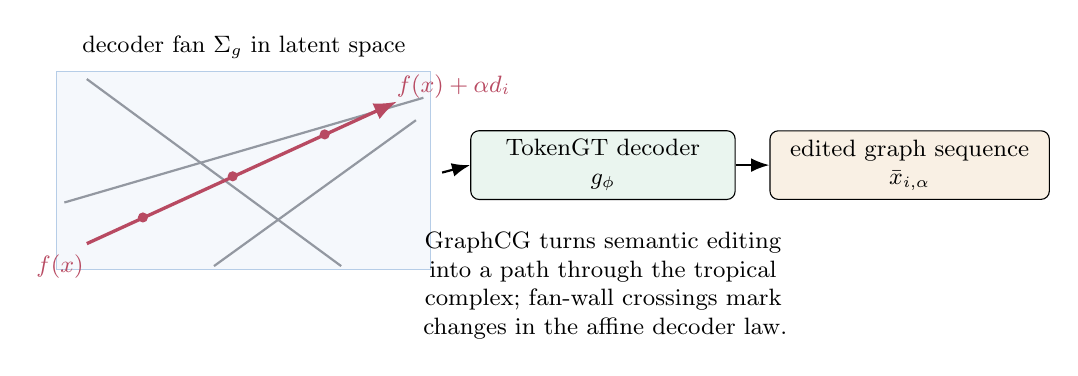
\begin{tikzpicture}[font=\small, >=Latex, scale=0.95, transform shape]
  \draw[fill=tokblue!5,draw=tokblue!35] (-2.5,-1.3) rectangle (2.5,1.35);
  \draw[tokgray!65,thick] (-2.4,-0.4) -- (2.4,1.0);
  \draw[tokgray!65,thick] (-2.1,1.25) -- (1.3,-1.25);
  \draw[tokgray!65,thick] (-0.4,-1.25) -- (2.3,0.7);
  \draw[tokrose,very thick,->] (-2.1,-0.95) -- (2.05,0.95);
  \filldraw[tokrose] (-1.35,-0.6) circle (1.7pt);
  \filldraw[tokrose] (-0.15,-0.05) circle (1.7pt);
  \filldraw[tokrose] (1.08,0.51) circle (1.7pt);
  \node[tokrose,below left=0.05cm and -0.03cm] at (-2.05,-0.92) {$f(x)$};
  \node[tokrose,above right=0.02cm and 0.02cm] at (1.9,0.85) {$f(x)+\alpha d_i$};
  \node[above=0.05cm] at (0,1.35) {decoder fan $\Sigma_g$ in latent space};
  \node[draw,rounded corners=3pt,fill=tokgreen!10,text width=3.3cm,align=center] (dec) at (4.8,0.1) {TokenGT decoder\\$g_\phi$};
  \draw[->,thick] (2.65,0.0) -- (dec.west);
  \node[draw,rounded corners=3pt,fill=tokamber!12,text width=3.5cm,align=center] (graphs) at (8.9,0.1) {edited graph sequence\\$\bar x_{i,\alpha}$};
  \draw[->,thick] (dec.east) -- (graphs.west);
  \node[below=0.3cm of dec,text width=6.2cm,align=center] {GraphCG turns semantic editing into a path through the tropical complex; fan-wall crossings mark changes in the affine decoder law.};
\end{tikzpicture}
\caption{GraphCG-style linear latent editing as tropical fan navigation.  The learned direction $d_i$ selects a one-dimensional slice through the decoder's TokenGT tropical complex.  This figure is a new schematic based on the GraphCG latent-editing mechanism of Liu et al. \cite{liu2024graphcg} and the fan viewpoint of Su and Liu \cite{su2026tropicalexpressivity}.}
\label{fig:graphcg-fanslice}
\end{figure}

\paragraph{Implication for the main thesis.}
GraphCG-style training changes TokenGT expressivity in a different register from edge tokenization.  Edge and vertex tokens enlarge the structural information and the tropical site count available to attention.  GraphCG then imposes a semantic coordinate system on the learned latent space.  The architecture may remain universal, but the trained model is encouraged to realize graph-to-graph maps that factor through a small number of controllable latent flows.  This is powerful for molecular and geometric graph editing, because one can traverse properties such as size, shape, or chemical score by varying $\alpha$; it is also a limitation, because arbitrary graph-to-graph maps need not admit a low-dimensional semantic-flow factorization.

\section{Edge Cases and Failure Modes for TokenGT Expressivity}

The positive results depend on assumptions.  This section lists the most important failure modes.

\begin{proposition}[Identifier rank bottleneck]
If the node identifiers $P_1,\dots,P_n$ are not linearly independent enough to separate equality patterns, then TokenGT may fail to approximate all equivariant basis tensors.
\end{proposition}

\begin{proof}
The basis-tensor construction requires dot products to implement equality tests.  If $P_a=P_b$ for $a\ne b$, then no dot-product score using only identifier coordinates can distinguish vertex $a$ from vertex $b$.  Any basis tensor whose support treats $a$ and $b$ differently cannot be implemented.  More generally, if the Gram matrix has off-diagonal entries too close to diagonal entries relative to available score margins, finite-temperature attention cannot robustly separate equality from inequality.
\end{proof}

\begin{proposition}[Key normalization can collapse power weights]
If all projected keys are normalized to the same norm, the power diagram of attention degenerates to an ordinary Voronoi or angular nearest-neighbor diagram.  Some weighted-cell configurations used in maximal tropical constructions are then unavailable.
\end{proposition}

\begin{proof}
The power weight associated with key $k_j$ is $\|k_j\|^2$.  If $\|k_j\|=R$ for all $j$, then all weights equal $R^2$ and cancel in power-distance comparisons.  The routing condition reduces to nearest-site comparison with equal weights, equivalently maximum cosine similarity when query norms are fixed.  Weighted power cells that require unequal $\|k_j\|^2$ cannot be realized.
\end{proof}

\begin{proposition}[Sparse token count need not improve the exponent]
Let $\cG_n$ be a graph family with $m(n)=O(n)$ edges.  Sparse TokenGT has the same tropical region exponent in $n$ as node-only sequence tokenization, despite having strictly richer graph information.
\end{proposition}

\begin{proof}
By \Cref{cor:sparse-edge}, $N_G=n+m+O(1)=O(n)$.  The region count $\Theta(N_G^{dL})$ is therefore $\Theta(n^{dL})$.  The expressivity gain is relational and constant-factor in this asymptotic measure, not exponent-changing.
\end{proof}

\begin{proposition}[Unlabeled non-equivariant targets are impossible]
No permutation-equivariant graph transformer, TokenGT included, can realize a non-equivariant function on unlabeled graphs.
\end{proposition}

\begin{proof}
If $G$ and $\pi G$ are the same unlabeled input, a well-defined graph-to-graph function must output isomorphic graphs with corresponding relabeling.  A non-equivariant target violates this.  Since TokenGT with orthonormal identifiers is constructed to be equivariant when identifiers are relabeled with vertices, it cannot assign incompatible outputs to two representatives of the same unlabeled graph.
\end{proof}

\section{Putting the Five Perspectives Together}

The five expressivity viewpoints now align as follows.

\begin{longtable}{>{\raggedright\arraybackslash}p{0.2\textwidth} >{\raggedright\arraybackslash}p{0.34\textwidth} >{\raggedright\arraybackslash}p{0.34\textwidth}}
\toprule
Perspective & Standard or naked transformer & TokenGT change \\
\midrule
\endhead
Functional approximation & Sequence transformers approximate continuous sequence maps; naked graph transformers without structure see bags of vertices. & Edge/vertex tokenization plus identifiers approximates equivariant graph-to-graph maps and interpolates finite graph maps with output slots. \\
\addlinespace
Boolean circuits & Hard attention is AC0-like under restrictions; saturated float attention is bounded by TC0. & Graph tokens expose adjacency and incidence bits, enabling threshold-circuit simulation over graph predicates with gate tokens. \\
\addlinespace
Tropical geometry & Zero-temperature attention partitions query space by power diagrams; multi-head attention uses Minkowski sums; regions scale like $\Theta(N^{dL})$. & Replace $N$ by graph-token count $N_G=n+m$ or $n^k$; incidence identifiers add equality-pattern routing fans. \\
\addlinespace
GraphCG-style training & Ordinary expressivity theorems do not constrain how learned graph edits are organized in latent space. & Semantic directions and step sizes select controllable graph-to-graph flows; in the tropical skeleton these are one-dimensional slices through the decoder fan. \\
\addlinespace
Toric geometry & ReLU subnets can be toric via rational fans; general softmax transformers are not fan support functions. & TokenGT inherits the conditional fan bridge only for zero-temperature rational CPWL skeletons; full graph self-attention with moving keys remains generally non-toric. \\
\bottomrule
\end{longtable}

\section{Conclusion}

TokenGT changes transformer expressivity by changing the object to which attention is applied.  Once edges and vertices are both tokens, the sequence length becomes a graph-dependent combinatorial quantity, and identifier dot products make incidence available to ordinary attention.  This yields universal approximation of equivariant graph-to-graph maps, exact finite interpolation with output slots, threshold-circuit simulations over graph predicates, and tropical region bounds governed by $N_G=n+m$ or $n^k$ rather than by vertex count alone.

The tropical view clarifies the geometry of this gain.  Edge tokenization increases the number of sites in the power diagram and the number of vertices available to head polytopes; multi-head attention then forms Minkowski sums, and depth compounds the resulting fan refinements.  The gain is largest for dense graphs and higher-order tokenization; it is mostly relational rather than exponent-changing for sparse bounded-degree families.

GraphCG-style training adds a complementary implication.  It does not enlarge the formal TokenGT architecture class by itself, but it changes which graph-to-graph maps are favored: maps that factor through semantic latent directions and step-size-controlled edit curves.  In the tropical skeleton, those edit curves are slices through the decoder's polyhedral fan, so controllable graph generation can be read as learned navigation through fan cells.  This perspective also exposes the caveats: contrastive condition consistency does not uniquely identify semantic factors, and low-dimensional latent directions cannot represent arbitrary graph edits without enough directions, nonlinear residual editing, or a decoder that folds the latent space.

The toric view is more delicate.  ReLU networks and zero-temperature rational CPWL skeletons admit fan and divisor interpretations, but general transformers do not.  Finite-temperature softmax is smooth, full self-attention has moving-key quadratic boundaries, biases break conical fan structure unless homogenized, normalization is non-CPWL, and signed values do not fit a naive logarithmic tropicalization.  Thus transformers do not universally sit at the intersection of toric and tropical geometry.  A precise statement is narrower and more useful: certain transformer skeletons have tropical normal fans, and when those fans are rational and support CPWL ReLU functions, toric geometry supplies divisors and polytopes that lift the tropical combinatorics.

\appendix

\section{Additional Proof Details}

\subsection{Softmax stability on graph-token cells}

Let $s\in\R^N$ and suppose $s_i\ge s_j+\delta$ for all $j\ne i$.  Write
\[
  P_\tau(s)=\tau\log\sum_j e^{s_j/\tau}.
\]
Then
\[
  P_\tau(s)
  =
  s_i+\tau\log\left(1+\sum_{j\ne i} e^{(s_j-s_i)/\tau}\right),
\]
so
\[
  0\le P_\tau(s)-s_i
  \le
  \tau\log(1+(N-1)e^{-\delta/\tau}).
\]
The gradient is the softmax vector $p$.  Since $p_i=1/(1+r)$ with $0\le r\le (N-1)e^{-\delta/\tau}$,
\[
  \|p-e_i\|_1=2(1-p_i)\le 2r\le 2(N-1)e^{-\delta/\tau}.
\]
The Hessian is
\[
  \nabla^2P_\tau(s)=\frac1\tau(\diag(p)-pp^\top).
\]
On the stable region, the total off-winner mass is at most $(N-1)e^{-\delta/\tau}$, and the covariance matrix $\diag(p)-pp^\top$ has spectral norm bounded by that mass up to an absolute constant; using the looser bound in \cite{su2026tropicalexpressivity} gives
\[
  \|\nabla^2P_\tau(s)\|_2\le \frac1\tau(N-1)e^{-\delta/\tau}.
\]
Replacing $N$ by $N_G$ gives the graph-token version.

\subsection{Finite interpolation by ReLU networks}

Let $z_1,\dots,z_M\in\R^D$ be distinct contextual codes for graphs in a finite domain.  Choose pairwise disjoint balls $B(z_r,\rho_r)$ with no other code inside.  A ReLU network can implement a tent function $\psi_r$ that equals $1$ at $z_r$ and $0$ at all $z_s$, $s\ne r$, by taking maxima of separating affine functions and clipping with ReLUs.  Then any table $y_r$ is represented on the finite set by
\[
  z\mapsto \sum_{r=1}^M y_r\psi_r(z).
\]
This is the lookup step used in \Cref{thm:finite-interp}.

\subsection{A dense-order version of the circuit theorem}

For dense order-$k$ tokenization, every input Boolean variable is already a token indexed by $i\in[n]^k$.  A threshold circuit over these variables is simulated exactly as in \Cref{thm:tc0-sim}.  The only change is that incoming-wire selection uses equality tests among $k$ identifier coordinates rather than endpoint tests among two coordinates.  Therefore the resource count is polynomial in $n^k$ for fixed $k$.

\section{Bibliography}

\begin{thebibliography}{99}

\bibitem{vaswani2017attention}
Ashish Vaswani, Noam Shazeer, Niki Parmar, Jakob Uszkoreit, Llion Jones, Aidan N. Gomez, Lukasz Kaiser, and Illia Polosukhin.
\newblock Attention is all you need.
\newblock In \emph{Advances in Neural Information Processing Systems}, 2017.

\bibitem{yun2020universal}
Chulhee Yun, Srinadh Bhojanapalli, Ankit Singh Rawat, Sashank J. Reddi, and Sanjiv Kumar.
\newblock Are transformers universal approximators of sequence-to-sequence functions?
\newblock In \emph{International Conference on Learning Representations}, 2020.
\newblock arXiv:1912.10077.

\bibitem{kim2022tokengt}
Jinwoo Kim, Tien Dat Nguyen, Seonwoo Min, Sungjun Cho, Moontae Lee, Honglak Lee, and Seunghoon Hong.
\newblock Pure transformers are powerful graph learners.
\newblock In \emph{Advances in Neural Information Processing Systems}, 2022.
\newblock arXiv:2207.02505.

\bibitem{su2026tropicalexpressivity}
Ye Su and Yong Liu.
\newblock Expressivity of transformers: A tropical geometry perspective.
\newblock arXiv:2604.14727, 2026.

\bibitem{hashemi2025tropicalattention}
Baran Hashemi, Kurt Pasque, Chris Teska, and Ruriko Yoshida.
\newblock Tropical attention: Neural algorithmic reasoning for combinatorial algorithms.
\newblock arXiv:2505.17190, 2025.

\bibitem{fu2025toricrelu}
Yaoying Fu.
\newblock Toric geometry of ReLU neural networks.
\newblock arXiv:2509.05894, 2025.

\bibitem{merrill2022saturated}
William Merrill, Ashish Sabharwal, and Noah A. Smith.
\newblock Saturated transformers are constant-depth threshold circuits.
\newblock \emph{Transactions of the Association for Computational Linguistics}, 10:843--856, 2022.
\newblock arXiv:2106.16213.

\bibitem{hahn2020limitations}
Michael Hahn.
\newblock Theoretical limitations of self-attention in neural sequence models.
\newblock \emph{Transactions of the Association for Computational Linguistics}, 8:156--171, 2020.
\newblock arXiv:1906.06755.

\bibitem{ahvonen2026logic}
Veeti Ahvonen, Maurice Funk, Damian Heiman, Antti Kuusisto, and Carsten Lutz.
\newblock Expressive power of graph transformers via logic.
\newblock arXiv:2508.01067v2, 2026.

\bibitem{alpay2026geometry}
Faruk Alpay and Bilge Senturk.
\newblock The geometry of thought: Disclosing the transformer as a tropical polynomial circuit.
\newblock arXiv:2601.09775, 2026.

\bibitem{zhang2018tropical}
Liwen Zhang, Gregory Naitzat, and Lek-Heng Lim.
\newblock Tropical geometry of deep neural networks.
\newblock In \emph{International Conference on Machine Learning}, pages 5824--5832, 2018.
\newblock arXiv:1805.07091.

\bibitem{maron2019invariant}
Haggai Maron, Heli Ben-Hamu, Nadav Shamir, and Yaron Lipman.
\newblock Invariant and equivariant graph networks.
\newblock In \emph{International Conference on Learning Representations}, 2019.

\bibitem{maron2019provably}
Haggai Maron, Heli Ben-Hamu, Haggai Serviansky, and Yaron Lipman.
\newblock Provably powerful graph networks.
\newblock In \emph{Advances in Neural Information Processing Systems}, 2019.

\bibitem{maron2019universality}
Haggai Maron, Ethan Fetaya, Nimrod Segol, and Yaron Lipman.
\newblock On the universality of invariant networks.
\newblock In \emph{International Conference on Machine Learning}, 2019.

\bibitem{keriven2019universal}
Nicolas Keriven and Gabriel Peyre.
\newblock Universal invariant and equivariant graph neural networks.
\newblock In \emph{Advances in Neural Information Processing Systems}, 2019.

\bibitem{kim2021hot}
Jinwoo Kim, Saeyoon Oh, and Seunghoon Hong.
\newblock Transformers generalize DeepSets and can be extended to graphs and hypergraphs.
\newblock In \emph{Advances in Neural Information Processing Systems}, 2021.
\newblock arXiv:2110.14416.

\bibitem{merrill2023cot}
William Merrill and Ashish Sabharwal.
\newblock The expressive power of transformers with chain of thought.
\newblock arXiv:2310.07923, 2023.

\bibitem{chiang2023logic}
David Chiang, Peter Cholak, and Anand Pillay.
\newblock Tighter bounds on the expressivity of transformer encoders.
\newblock In \emph{International Conference on Machine Learning}, 2023.

\bibitem{strobl2024survey}
Lena Strobl, William Merrill, Gail Weiss, David Chiang, and Dana Angluin.
\newblock What formal languages can transformers express? A survey.
\newblock \emph{Transactions of the Association for Computational Linguistics}, 2024.

\bibitem{maclagan2015tropical}
Diane Maclagan and Bernd Sturmfels.
\newblock \emph{Introduction to Tropical Geometry}.
\newblock American Mathematical Society, 2015.

\bibitem{fulton1993toric}
William Fulton.
\newblock \emph{Introduction to Toric Varieties}.
\newblock Princeton University Press, 1993.

\bibitem{cox2011toric}
David A. Cox, John B. Little, and Henry K. Schenck.
\newblock \emph{Toric Varieties}.
\newblock American Mathematical Society, 2011.

\bibitem{gritzmann1993minkowski}
Peter Gritzmann and Bernd Sturmfels.
\newblock Minkowski addition of polytopes: Computational complexity and applications to Groebner bases.
\newblock \emph{SIAM Journal on Discrete Mathematics}, 6(2):246--269, 1993.

\bibitem{ziegler1995polytopes}
Gunter M. Ziegler.
\newblock \emph{Lectures on Polytopes}.
\newblock Springer, 1995.

\bibitem{zaslavsky1975arrangements}
Thomas Zaslavsky.
\newblock Facing up to arrangements: Face-count formulas for partitions of space by hyperplanes.
\newblock \emph{Memoirs of the American Mathematical Society}, 1(154), 1975.

\bibitem{montufar2014regions}
Guido Montufar, Razvan Pascanu, Kyunghyun Cho, and Yoshua Bengio.
\newblock On the number of linear regions of deep neural networks.
\newblock In \emph{Advances in Neural Information Processing Systems}, 2014.

\bibitem{serra2018bounding}
Thiago Serra, Christian Tjandraatmadja, and Srikumar Ramalingam.
\newblock Bounding and counting linear regions of deep neural networks.
\newblock In \emph{International Conference on Machine Learning}, 2018.

\bibitem{hanin2019complexity}
Boris Hanin and David Rolnick.
\newblock Complexity of linear regions in deep networks.
\newblock In \emph{International Conference on Machine Learning}, 2019.

\bibitem{aurenhammer1987power}
Franz Aurenhammer.
\newblock Power diagrams: Properties, algorithms and applications.
\newblock \emph{SIAM Journal on Computing}, 16(1):78--96, 1987.

\bibitem{litvinov2007maslov}
Grigori L. Litvinov.
\newblock The Maslov dequantization, idempotent and tropical mathematics: A brief introduction.
\newblock arXiv:math/0507014, 2005.

\bibitem{liu2024graphcg}
Shengchao Liu, Chengpeng Wang, Jiarui Lu, Weili Nie, Hanchen Wang, Zhuoxinran Li, Bolei Zhou, and Jian Tang.
\newblock Unsupervised discovery of steerable factors when graph deep generative models are entangled.
\newblock \emph{Transactions on Machine Learning Research}, 2024.
\newblock arXiv:2401.17123.

\end{thebibliography}

\end{document}
